\newcommand{\Ca}{\ensuremath{\mbox{Ca}^{2+}}\xspace}
\newcommand{\CaC}{\ensuremath{\left[\mbox{Ca}^{2+}\right]}\xspace}
\newcommand{\Na}{\ensuremath{\mbox{Na}^{+}}\xspace}
\newcommand{\Cl}{\ensuremath{\mbox{Cl}^{-}}\xspace}
\newcommand{\Mg}{\ensuremath{\mbox{Mg}^{2+}}\xspace}
\newcommand{\MgC}{\ensuremath{\left[\mbox{Mg}^{2+}\right]}\xspace}
\newcommand{\PEe}{\mathrm{PE}_{\mathrm{e}}}
\newcommand{\T}{\ensuremath{\mathcal{T}}\xspace}

% positional numbers
\newcommand{\kth}{\ensuremath{k^{\scriptscriptstyle\text{th}}}\xspace}
\newcommand{\nth}{\ensuremath{n^{\scriptscriptstyle\text{th}}}\xspace}

\newcommand{\Ltwo}[1]{\ensuremath{\|#1\|_{L^2}\xspace}}

\newcommand{\Dt}{\ensuremath{\Delta{}t}}
\newcommand{\Ds}{\ensuremath{\Delta{}s}}
\newcommand{\diff}[2][{}]{\dfrac{\partial #1}{\partial #2}}

%\newcommand{\citet}[1]{\cite{#1}}

\fenicschapter{A coupled stochastic and deterministic model of \Ca dynamics in the dyadic cleft}
              {A coupled stochastic and deterministic model of \Ca dynamics in the dyadic cleft}
              {Johan Hake}
              {hake}

\section{Introduction}
\label{sec:intro}
From the time we are children, we are told that we should drink milk because it is an important source of calcium (\Ca), and that \Ca is vital for a strong bone structure. What we do not hear as frequently, is that \Ca is one of the most important cellular messengers in the human body \cite{AlbertsBrayLewisEtAl2002}. In particular, \Ca controls cell death, neural signaling, secretion of different chemical substances to the body, and the focus of this chapter: the contraction of cells in the heart.\par

In this chapter, we will present a computational model that can be used to model \Ca dynamics in a small sub-cellular domain called the dyadic cleft. The model includes \Ca diffusion, which is described by an advection-diffusion partial differential equation, and discrete channel dynamics, which is described by stochastic Markov models. Numerical methods implemented in \pydolfin solving the partial differential equation will also be pregsented. In the last section, we describe a time stepping scheme that is used to solve the stochastic and deterministic models. We will also present a solver framework, \texttt{diffsim}, that implements the time stepping scheme together with the numerical methods solving the computational model described above.\par

\section{Biological background}
\index{sarcoplasmic reticulum}
\index{ryanodine receptor}
%\index{L-type Ca channels}
\index{cell membrane}
\index{excitation contraction coupling}
\index{cytosole}
In a healthy heart, every heart beat originates in the sinusoidal node, where pacemaker cells trigger an electric signal. This signal is a difference in electric potential between the interior and exterior of the heart cells. These two domains are separated by the cell membrane. The difference in the electric potential between these domains is called the membrane potential. The membrane potential propagates through the whole heart using active conductances at the cell membrane. The actively propagating membrane potential is called an action potential. When an action potential arrives at a heart cell, it triggers the L-type \Ca channels (LCCs). These channels bring \Ca into the cell. Some of the \Ca diffuse over a small cleft, called the dyadic cleft, and cause further \Ca release from an intracellular \Ca storage, the sarcoplasmic reticulum (SR), through a channel called the ryanodine receptor (RyR). The \Ca ions then diffuse to the main intracellular domain of the cell, the cytosole, in which the contractile proteins are situated. The \Ca ions attach to these proteins and trigger contraction. The strength of the contraction is controlled by the strength of the \Ca concentration (\CaC) in cytosole. The contraction is succeeded by a period of relaxation, which is caused by the extraction of \Ca from the intracellular space by various proteins. \par

This chain of events is labelled the Excitation Contraction (EC) coupling \cite{Bers2001}. Several severe heart diseases can be related to impaired EC coupling. By broadening the knowledge of the coupling, it may be possible to develop better treatments for such diseases. Although the big picture of EC coupling is straightforward to grasp, it involves the nonlinear action of hundreds of different protein species. Computational methods have emerged as a natural complement to experimental studies to better understand the intriguing coupling. In this chapter, we focus on the initial phase of the EC coupling, the stage where \Ca flows into the cell and triggers further \Ca release.\par

\newcommand{\figheight}{3.5cm}
\begin{figure}[t]
  \centering
  \begin{minipage}[t]{0.35\linewidth}
    \large \textbf{A}\\
    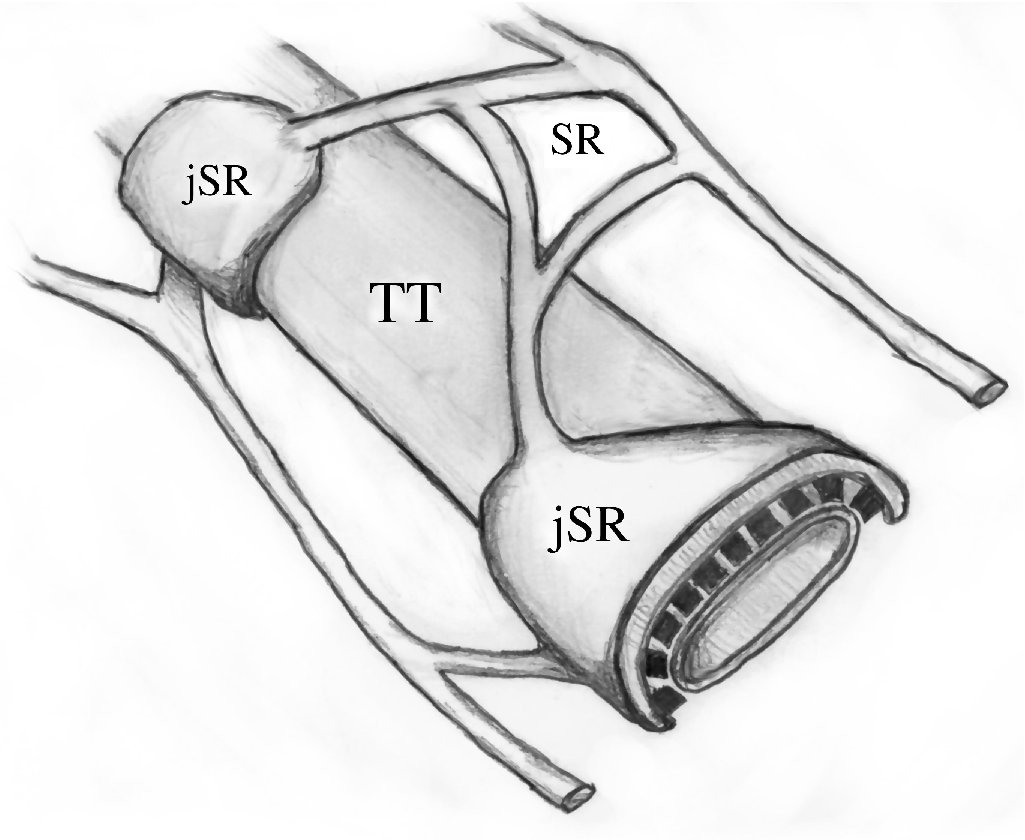
\includegraphics[width=\linewidth]{chapters/hake/pdf/SR_TT}
  \end{minipage}
  \begin{minipage}[t]{0.64\linewidth}
    \large \textbf{B}\\
    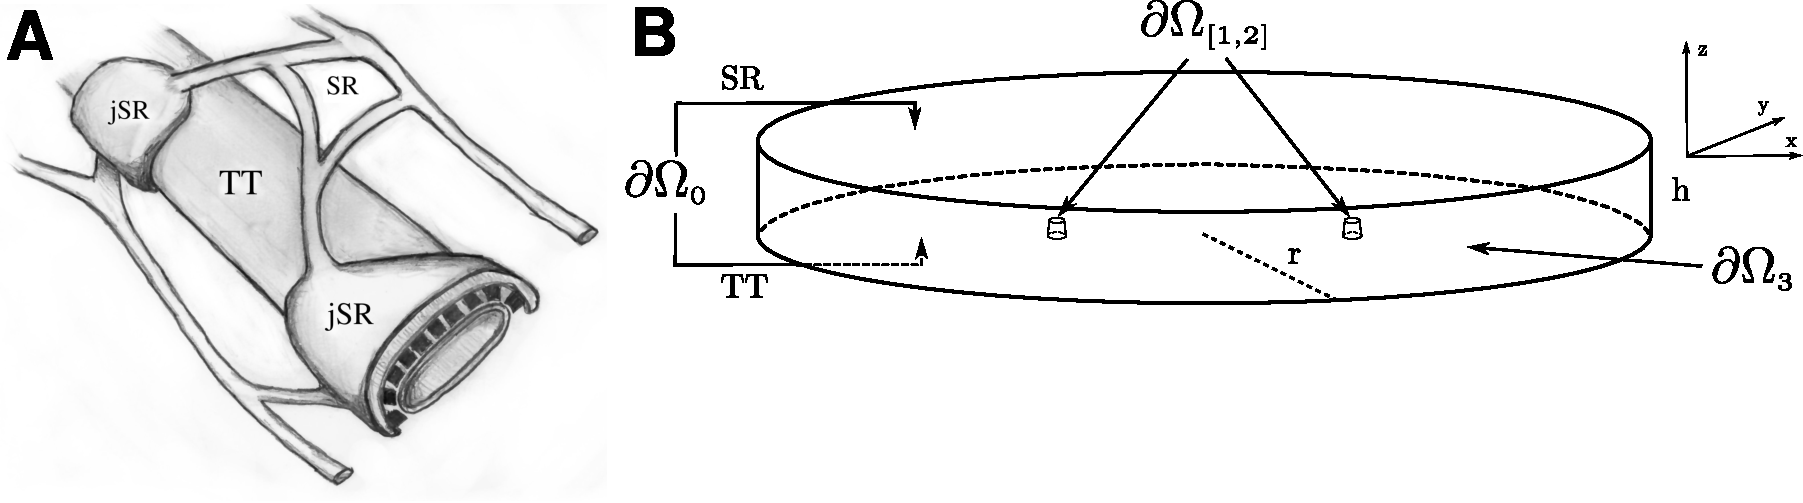
\includegraphics[width=\linewidth]{chapters/hake/pdf/disk}
  \end{minipage}
  \caption{\textbf{A}: A diagram showing the relationship between the TT, the SR, and the jSR. The volume between the flat jSR and the TT is the dyadic cleft. The black structures in the cleft are Ryanodine receptors, which are large channel proteins. \textbf{B}: The geometry used for the dyadic cleft. The top of the disk is the cell membrane of the SR or jSR. The bottom is the cell membrane of the TT, and the circumference of the disk is the interface to the cytosole. The elevations in the TT membrane models two ions channels.}
\label{fig:morphology}
\end{figure}

\section{Mathematical models}
\label{sec:mathematical-models}
In this section we describe the computational model for the early phase of the EC coupling. We first present the morphology of the cleft, and how we model this in our study. Then we describe the mathematical equation for the diffusion of \Ca inside the cleft together with the boundary fluxes. Finally, we discuss the stochastic models that govern the discrete channel dynamics of the LCCs and RyRs.\par

\subsection*{Morphology}
\label{sec:morphology}
\index{cell membrane}
\index{dyadic cleft}
\index{t-tubule}
\index{diffusion constant}
The dyadic cleft is the volume between a structure called the t-tubule (TT) and the SR. The TT is a network of pipe-like invaginations of the cell membrane that perforate the heart cell \cite{SoellerCannell1999}. In Fig.~\ref{fig:morphology} \textbf{A}, a sketch of a small part of a single TT together with a piece of SR is presented. Here we see that the junctional SR (jSR) is wrapped around the TT. The small volume between these two structures is the dyadic cleft. The space is not well defined as it is crowded with channel proteins, and its size also varies. In computational studies, it is commonly approximated as a disk or a rectangular slab \cite{PeskoffPostLanger1992,SoellerCannell1997,KohSrinivasanEtAl2006,TanskanenGreensteinEtAl2007}. In this study a disk with height, $h$ = 12 nm and radius, $r$ = 50 nm has been used for the domain $\Omega$, see Fig.~\ref{fig:morphology} \textbf{B}. The diffusion constant of \Ca is set to $\sigma$ = $10^5$ nm$^2$ ms$^{-1}$ \cite{LangerPeskoff1996}.\par

\subsection*{\Ca Diffusion}
\label{sec:ca-diffusion}

\paragraph*{Electro-Diffusion}
\index{Fick's second law}
\index{screening}
\index{electro-diffusion}
\index{advection-diffusion}
\index{Gouy-Chapman}
\index{Nernst-Planck equation}
We will use Fick's second law to model the diffusion of \Ca in the dyadic cleft. Close to the cell membrane, the ions are affected by an electric potential. The potential is caused by negative charges on the membrane \cite{McLaughlinSzaboEisenman1971,LangnerCafisoEtAl1990}. The potential attenuates fast as it is screened by the ions in the intracellular solution. We will describe the electric potential using the Gouy-Chapman method \cite{Grahame1947}. This theory introduces an advection term to the standard diffusion equation, which makes the resulting equation harder to solve. To simplify the presentation we will use a non-dimensional electric potential $\psi$, which is the electric potential scaled by a factor of $e/kT$. Here $e$ is the electron charge, $k$ is Boltzmann's constant and $T$ is the temperature. We will also use a non-dimensional electric field which is given by:
\begin{equation}
  \label{eq:electric_field}
  E=-\nabla\psi.
\end{equation}

The \Ca flux in a solution in the presence of an electric field is governed by the Nernst-Planck equation,
\begin{equation}
  \label{eq:nernst-planck}
  J = -\sigma\left(\nabla c-2\,cE\right),
\end{equation}
where $c = c(x,t)$ is the \CaC ($x\in\Omega$ and $t\in$[0,T]), $\sigma$ the diffusion constant, $E = E(x)$ the non-dimensional electric field and 2 is the valence of \Ca. Assuming conservation of mass, we arrive at the advection-diffusion equation,
\begin{equation}
  \label{eq:advection-diffusion}
  \dot{c}=\sigma\left(\Delta c - \nabla\cdot\left(2\,cE\right)\right).
\end{equation}
Here $\dot{c}$ is the time derivative of $c$.\par

The strength of $\psi$ is defined by the amount of charge at the cell membrane and by the combined screening effect of all the ions in the dyadic cleft. In addition to \Ca, the intracellular solution also contains \ensuremath{\mbox{K}^{+}}, \Na, \Cl, and \Mg. Following the previous approach by \citet{LangnerCafisoMarceljaEtAl1990} and \citet{SoellerCannell1997}, these other ions will be treated as being in steady state. The cell membrane is assumed to be planar and effectively infinite. This assumption allows us to use an approximation of the electric potential in the solution,
\begin{equation}
  \label{eq:electric_potential}
  \psi(z) = \psi_0\e^{-\kappa{}z}.
\end{equation}
Here $\psi_0$ is the non-dimensional potential at the membrane, $\kappa$ the inverse Debye length and $z$ the distance from the cell membrane. We will use $\psi_0=-2.2$ and $\kappa=1$ nm.\par

\paragraph*{Boundary fluxes}
\index{stochastic channel}
\index{t-tubule}
\index{sarcoplasmic reticulum}
\index{ryanodine receptor}
%\index{L-type Ca channels}
\index{cytosole}

The boundary, $\partial\Omega$, is divided into 4 disjoint boundaries, $\partial\Omega_k$, for $k=1,\ldots,4$, see Fig.~\ref{fig:morphology} \textbf{B}. To each boundary we associate a flux, $J_{|\partial\Omega_k}=J_k$. The SR and TT membranes are impermeable for ions, effectively making $\partial\Omega_{\scriptscriptstyle\text{1}}$, in Fig.~\ref{fig:morphology} \textbf{B}, a no-flux boundary, giving us,
\begin{equation}
  \label{eq:no-flux}
  J_{\scriptscriptstyle 1}= 0.
\end{equation}
We include 2 LCCs in our model. The \Ca flows into the cleft at the $\partial\Omega_{\scriptscriptstyle\text{[2,3]}}$ boundaries, see Fig.~\ref{fig:morphology} \textbf{B}. \Ca entering these channels then diffuse to the RyRs triggering \Ca release from the SR. This additional \Ca flux will not be included in the simulations. However, the stochastic dynamics of the opening of the channel will be included. Further detailes are presented in Section \ref{sec:stochastic-models} below. The \Ca that enters the dyadic cleft diffuses into the main compartment of cytosole, introducing a third flux. This flux is included in the model at the $\partial\Omega_{\scriptscriptstyle\text{3}}$ boundary.\par

The LCC is a stochastic channel that takes the state of either open or closed. When the channel is open, \Ca flows into the cleft. The dynamic that describe the stochastic behaviour is presented in Section \ref{sec:stochastic-models} below. The current amplitude of an open LCC channel is modelled to -0.1 pA \cite{GuiaSternLakattaEtAl2001}. The LCC flux is then,
%or as a Voltage and \CaC dependent current, using the constant field approximation \cite{Luo_1994_1071,Camp_1988_267}. The first flux is given by,
\begin{equation}
\label{eq:constant-current-flux}
J_{\scriptscriptstyle[2,3]}= \left\{
  \begin{array}{c@{\quad:\quad}l}
    0& \text{closed channel}\\
    - \frac{i}{2\,F\,A},& \text{open channel}
  \end{array}
\right.
\end{equation}
\noindent where $i$ is the amplitude, 2 the valence of \Ca, $F$ Faraday's constant and $A$ the area of the channel. Note that an inward current is by convention negative.\par
The flux to the cytosole is modeled as a concentration dependent flux,
\begin{equation}
  \label{eq:conc-dependent-flux}
  J_{\scriptscriptstyle 4}= -\sigma\frac{c - c_0}\Ds,
\end{equation}
where $c$ is the concentration in the cleft at the boundary, $c_0$ the concentration in the cytosole, and \Ds is an approximation of the distance to the center of the cytosole. In our model we have used \Ds = 50 nm.\par

\renewcommand{\figheight}{3cm}
\begin{figure}[t]
  \centering
  \begin{minipage}{0.79\linewidth}
    \fontfamily{cmss} \large \textbf{A}\\[0.5em]
    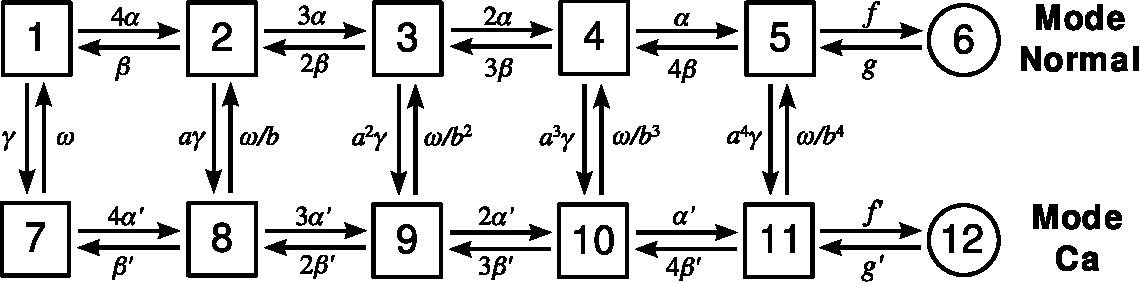
\includegraphics[height=\figheight]{chapters/hake/pdf/Jafri_1998_LCC_model}
  \end{minipage}
  \begin{minipage}{0.2\linewidth}
    \fontfamily{cmss} \large \textbf{B}\\[0.5em]
    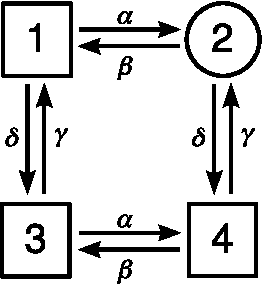
\includegraphics[height=\figheight]{chapters/hake/pdf/Stern_1999_RyR_model}
  \end{minipage}
\caption{\textbf{A}: State diagram of the discrete LCC Markov model from \citet{JafriRiceWinslow1998}. Each channel can be in one of the 12 states.  The transitions between the states are controlled by propensities. The $\alpha$, and $\beta$ are voltage dependent, $\gamma$ is \CaC dependent and $f$, $a$, $b$, and $\omega$ are constant, see \citet{JafriRiceWinslow1998} for further details. The channels operate in two modes: \textit{Mode normal}, represented by the states in the upper row, and \textit{Mode Ca}, represented the states in the lower row. In state 6 and 12 the channel is open, but state 12 is rarely entered as $f'\ll{}f$, effectively making \textit{Mode Ca} an inactivated mode.
\textbf{B}: State diagram of an RyR from \citet{SternSongChengEtAl1999}. The $\alpha$ and $\gamma$ propensities are \Ca dependent, representing the activation and inactivation dependency of the cytosolic \CaC. The $\beta$ and $\delta$ propensities are constant.}
\label{fig:markov-models}
\end{figure}

\subsection*{Stochastic models of single channels}
\label{sec:stochastic-models}
\index{stochastic channel}
\index{Markov chain model}
\index{Discrete state}
\index{propensity functions}
Discrete and stochastic Markov chain models are used to describe single channel dynamics. Such models are described by a certain number of discrete states. Each channel can be in either one of these states. A transition between two states is a stochastic event. The frequency of these events are determined by the propensity functions associated with each transition. These functions, which may vary with time, characterize the probability per unit time that the corresponding transition event occurs. Each Markov model defines its own propensity functions. \par

\paragraph*{L-type \Ca channel}
\label{sec:lcc}
%\index{L-type Ca channels}
The LCC opens when an action potential arrives at the cell. The channel inactivates when single \Ca ions bind to binding sites on the intracellular side of the channel. An LCC is composed of a complex of four transmembrane subunits. Each of these can be permissive or non-permissive. For the whole channel to be open, all four subunits need to be permissive and the channel then has to undergo a last conformational change to an opened state \cite{Hille2001}. In this chapter we are going to use a Markov model of the LCC that incorporates a voltage dependent activation together with a \Ca dependent inactivation \cite{JafriRiceWinslow1998,Gree_2002_2918}. The state diagram of this model is presented in Fig.~\ref{fig:markov-models} \textbf{A}. It consists of 12 states, where state 6 and 12 are the only conducting states, hence defineing the open states. The transition propensities are defined by a set of functions and constants, which are all described in \citet{GreensteinWinslow2002}.\par

\paragraph*{Ryanodine Receptors}
\label{sec:ryr}
\index{ryanodine receptor}
RyRs are \Ca specific channels that are gathered in clusters at the SR membrane in the dyadic cleft. These clusters can consist of several hundreds of RyRs \cite{BeuckelmannWier1988,Franzini-ArmstrongProtasiEtAl1999}. They open by single \Ca ions attaching to the receptors at the cytosolic side. We will use a modified version of a phenomenological RyR model that mimics the physiological functions of the channel \cite{SternSongChengEtAl1999}. The model consists of four states where only one is conducting, state 2, see Fig.~\ref{fig:markov-models} \textbf{B}. The $\alpha$ and $\gamma$ propensities are \Ca dependent, representing the activation and inactivation dependency of cytosolic \CaC. The $\beta$ and $\delta$ propensities are constants. For specific values for the propensities, see \citet{SternSongChengEtAl1999}.\par

\section{Numerical methods for the continuous system}
In this section, we will describe the numerical methods used to solve the continuous part of the computational model of the \Ca dynamics in the dyadic cleft. We will provide \pydolfin code for each part of the presentation. The first part of the section describes the discretization of the continuous problem using a finite element method. The second part describes a method to stabilize the discretization. In this part, we also conduct a parameter study to find the optimal stabilization parameters.\par
\begin{figure}
  \centering
  \LVerbatimInput[fontsize=\scriptsize,frame=lines,
  framerule=0.4mm,
  xleftmargin=10mm,xrightmargin=15mm,
  numbers=left,numbersep=5pt]{chapters/hake/code/matrix_assemble.py}
  \vspace{-1.5em}
  \caption{Python code for the assembly of the matrices and vectors from Eq.~(\ref{eq:matrices})-(\ref{eq:vector}).}
  \label{fig:assembly-algorithm}
\end{figure}

\subsection*{Discretization}
\label{sec:discretization}
The continuous problem is defined by Eqs.~(\ref{eq:advection-diffusion}~-\ref{eq:conc-dependent-flux}) together with an initial condition. Given a bounded domain $\Omega \subset \Rset^3$ with the boundary, $\partial\Omega$, we want to find $c = c(x,t) \in \Rset_+$, for $x\in \Omega$ and $t \in [0,T]$, such that:
\begin{equation}
%\renewcommand{\arraystretch}{1.5}
%\renewcommand{\baselinestretch}{1.5}
\label{eq:full_system}
\left\{
  \begin{array}{r@{\quad=\quad}ll}
    \dot{c}&\sigma\Delta c - \nabla\cdot\left(ca\right)&  \text{in } \Omega \\
    \sigma\partial_nc-ca\cdot n&J_k& \text{on } \partial\Omega_k,\; k = 1,\ldots,4,
  \end{array}
\right.
%\renewcommand{\arraystretch}{1}
%\renewcommand{\baselinestretch}{1}
\end{equation}
and $c(\cdot,0) = c_0(x)$. Here $a=a(x)=2\sigma E(x)$ and $J_k$ is the \kth flux at the \kth boundary $\partial\Omega_k$, where $\bigcup^4_{k=1}\partial\Omega_k=\partial\Omega$, $\partial_nc = \nabla c\cdot n$, where $n$ is the outward normal on the boundary. The $J_k$ are given by Eqs.~(\ref{eq:no-flux})-~(\ref{eq:conc-dependent-flux}).\par

The continuous equations are discretized using a finite element method in space. Eq.~(\ref{eq:full_system}) is multiplied with a proper test function $v$, and integrated over the spatial domain, thus obtaining:
\begin{equation}
  \label{eq:advection-diffusion-weak-form-0}
  \int_\Omega\dot{c}v\,dx = \int_\Omega \left(\sigma\Delta c-\nabla(ca)\right) v\,dx.
\end{equation}
Integration by parts, together with the boundary conditions in Eq.~(\ref{eq:full_system}), yield:
\begin{equation}
  \label{eq:advection-diffusion-weak-form}
  \int_\Omega\dot{c}v\,dx = -\int_\Omega \left(\sigma\nabla c-ca\right)\cdot\nabla v\,dx + \sum_k\int_{\partial\Omega_k} J_kv\,ds_k.
\end{equation}
Consider a mesh \T = $\left\{K\right\}$ of simplicial elements $K$. Let $V_h$ denote the space of piecewise linear polynomials, defined relative to the mesh \T. Using the backward Euler methods in time, we seek an approximation of $c$: $c_h\in V_h$ with nodal basis $\left\{\phi_i\right\}^N_{i=1}$. Eq.~(\ref{eq:advection-diffusion-weak-form}) can now be discretized as follows: Consider the \nth time step, then given $c_h^n$ find $c_h^{n+1} \in V_h$ such that
\begin{equation}
  \label{eq:advection-diffusion-weak-discrete-form}
  \int_{\Omega} \frac{c_h^{n+1}-c_h^{n}}{\Dt}v\,dx = -\int_{\Omega} \left(\sigma\nabla c_h^{n+1}-c_h^{n+1}a\right)\cdot\nabla v\,dx + \sum_k\int_{\partial\Omega} J_kv\,ds_{k}\quad\forall v \in V_h,
\end{equation}
where \Dt is the size of the time step. The trial function $c^n_h(x)$ is expressed as a weighted sum of basis functions,
\begin{equation}
  \label{eq:discrete-solution}
  c^n_h(x) = \sum^N_j C_j^n\phi_j(x).
\end{equation}
where $C_j^n$ are the coefficients. Due to the choice of $V_h$ will the number of unknowns, $N$, coincide with the number of vertices of the mesh.\par

\begin{figure}
  \centering
  \LVerbatimInput[fontsize=\scriptsize,frame=lines,
  framerule=0.4mm,
  xleftmargin=10mm,xrightmargin=15mm,
  numbers=left,numbersep=5pt]{chapters/hake/code/stabilization.py}
  \vspace{-1.5em}
  \caption{Python code for the assembly of the SUPG term for the mass and advection matrices.}
  \label{fig:SUPG-assembly-algorithm}
\end{figure}
Taking test functions, $v=\phi_i$, $i\in\left\{1,\ldots,N\right\}$, gives the following algebraic system of equations in terms of the coefficients $\left\{ c^{n+1}_i\right\}^N_{i=1}$.
\begin{equation}
  \label{eq:algebraic-equation}
  \frac{1}{\Dt}\text{\bfseries\itshape M}\left(C^{n+1}-C^n\right) =  \left(-\text{\bfseries\itshape K}+\text{\bfseries\itshape E}+\sum_k\alpha^k\text{\bfseries\itshape F}^k\right)C_j^{n+1}+\sum_k c_0^k\,f^k.
\end{equation}
Here $C^n\in \Rset^N$ is the vector of coefficients from the discrete solution $c^n_h(x)$, $\alpha^k$ and $c_0^k$ are constant coefficients given by Eqs.~(\ref{eq:no-flux})~-~(\ref{eq:conc-dependent-flux}) and\\[-1.0em]
\begin{equation}
  \renewcommand{\arraystretch}{1.7}
  \renewcommand{\baselinestretch}{1.7}
  \begin{array}{r@{\;=\;}lcr@{\;=\;}l}
    \text{\bfseries\itshape M}_{ij}&\displaystyle\int_\Omega\phi_i\phi_jdx,& \quad\quad&\text{\bfseries\itshape K}_{ij}&\displaystyle\int_\Omega\nabla\phi_i\cdot\nabla\phi_jdx,\\
    \text{\bfseries\itshape E}_{ij}&\displaystyle\int_\Omega a\phi_i\cdot\nabla\phi_jdx,& \quad\quad&\text{\bfseries\itshape F}^k_{ij}&\displaystyle\int_{\partial\Omega_k}\phi_i\phi_jds,
  \end{array}
  \renewcommand{\arraystretch}{1}
  \renewcommand{\baselinestretch}{1}
  \label{eq:matrices}
\end{equation}
are the entries in the {\bfseries\itshape M}, {\bfseries\itshape K}, {\bfseries\itshape E} and {\bfseries\itshape F}$^k$ matrices. $f^k$ are boundary source vectors corresponding to the \kth boundary. The vector elements are given by:
\begin{equation}
  \label{eq:vector}
  f^k_{i}=\int_{\partial\Omega_k}\phi_ids.
\end{equation}
%Note that $a$ is a function given by a finite element vector space. In Section \ref{sec:results} we will show the impact different orders of this space has on the final result.\par

The \pydolfin code for the assembly of the matrices and vectors in Eqs.~(\ref{eq:matrices})-(\ref{eq:vector}) is presented in Fig. \ref{fig:assembly-algorithm}. Note that we define only one form for the different boundary mass matrices and boundary source vectors, \texttt{u*v*ds} and \texttt{v*ds} respectively. The \texttt{assemble} routine will assemble these forms over the $0^{\scriptscriptstyle\text{th}}$ sub-domain, see line 31 and 33 in Fig. \ref{fig:assembly-algorithm}. By passing sub domain specific \texttt{MeshFunction}s to the assemble routine we can assemble the correct boundary mass matrices and boundary source vectors. We collect the matrices and boundary source vectors. These are then added to form the linear system to be solved at each time step. If an LCC opens, we get contributions to the right-hand side from the source vectors. If an LCC closes, the same source vectors are removed from the right-hand side. When an LCC either opens or closes, a large flux is either added or removed from the system. To be able to resolve the sharp time gradients correctly, we need to take smaller time steps after such an event. The time step is then expanded by multiply it with a constant > 1.\par

The sparse linear system is solved using the \petsc linear algebra backend \cite{BalayBuschelmanGroppEtAl2001} in \pydolfin together with the Bi-CGSTAB iterative solver \cite{Vorst1992}, and the BoomerAMG preconditioners from hypre \cite{FalgoutYang2002}. In Fig.~\ref{fig:solving-algorithm}, a script is presented that solves the algebraic system from Eq.~(\ref{eq:algebraic-equation}) together with a crude time stepping scheme for the opening and closing of the included LCC channel.\par

\subsection*{Stabilization}
\label{sec:stabilization}
\index{stabilization}
\index{stabilization!Streamline upwind Petrov-Galerkin}
\index{stabilization!parameter}
\index{stabilization!element P\'eclet number}
\index{tetgen}

It turns out that the algebraic system in Eq.~(\ref{eq:algebraic-equation}) can be numerically unstable for physiological relevant values of $a$. This is due to the transport term introduced by {\bfseries\itshape E}$_{ij}$ from Eq.~(\ref{eq:matrices}). We have chosen to stabilize the system using the Streamline upwind Petrov-Galerkin (SUPG) method \cite{BrooksHughes1982}. This method adds an upwind discontinuous contribution to the testfunction in the streamline direction Eq.~(\ref{eq:advection-diffusion-weak-form-0}),
\begin{equation}
  \label{eq:stabilizing-term}
  v' = v+s, \text{ where } s = \tau\frac{h\tau_e}{2\|a\|}a\cdot\nabla v.
\end{equation}
Here $\tau$ is a parameter we want to optimize (see later in this Section), $\|\cdot\|$ is the Euclidian norm in $\Rset^3$, $h=h(x)$ is the element size, and $\tau_e=\tau_e(x)$, is given by,
\begin{equation}
  \label{eq:element-tau}
  \tau_e=\coth(\PEe)-\frac{1}{\PEe},
\end{equation}
where $\PEe$ is the element P\'eclet number:
\begin{equation}
  \label{eq:peclet}
  \PEe = \frac{\|a\|h}{2\sigma}.
\end{equation}
When $\PEe$ is larger than 1 the system become unstable, and oscillations is introduced.\par

In the 1D case, with a uniform mesh, the stabilization term defined by Eqs.~(\ref{eq:element-tau})~-~(\ref{eq:peclet}), can give nodal exact solutions \cite{ChristieGriffithsMitchellEtAl1976,BrooksHughes1982}. Our choice of stabilization parameter is inpired by this. We have used the diameter of the sphere that circumscribes the local tetrahedron as $h$. This is what \dolfin implements in the function \texttt{Cell.diameter()}. We recognize that other choices exist, which might give better stabilization \cite{JohnKnobloch2007}. \citet{TezduyarPark1986} use a length based on the size of the element in the direction of $a$.\par

The \pydolfin code that assembles the SUPG part of the problem is presented in Fig.~\ref{fig:SUPG-assembly-algorithm}. In the script, two matrices, \texttt{E\_stab} and \texttt{M\_stab} are assembled. Both matrices are added to the corresponding advection and mass matrices \texttt{E} and \texttt{M}, weighted by the global parameter \texttt{tau}.\par

A mesh with finer resolution close to the TT surface, at $z=0$ nm, is used to resolve the steep gradient of the solution in this area. It is here the electric field is at its strongest, yielding an element P\'eclet number larger than 1. However the field attenuate fast: at $z=3$ nm the field is down to 5\% of the maximal amplitude, and at $z=5$ nm, it is down to 0.7\%.The mesh can thus be fairly coarse in the interior of the domain. The mesh generator \texttt{tetgen} is used to to produce meshes with the required resolution \cite{Si2007}.\par

\begin{figure}
  \centering
  \LVerbatimInput[fontsize=\scriptsize,frame=lines,
  framerule=0.4mm,
  xleftmargin=10mm,xrightmargin=15mm,
  numbers=left,numbersep=5pt]{chapters/hake/code/solving.py}
  \vspace{-1.5em}
  \caption{Python code for solving the system in Eq.~(\ref{eq:algebraic-equation}), using the assembled matrices from the two former code examples from Fig.~\ref{fig:assembly-algorithm}-~\ref{fig:SUPG-assembly-algorithm}.}
  \label{fig:solving-algorithm}
\end{figure}

\newcommand{\leftfigsize}{0.66\linewidth}
\newcommand{\rightfigsize}{0.31\linewidth}

\begin{figure}[t]
    \begin{minipage}[t]{\leftfigsize}
      \raisebox{-3.45cm}{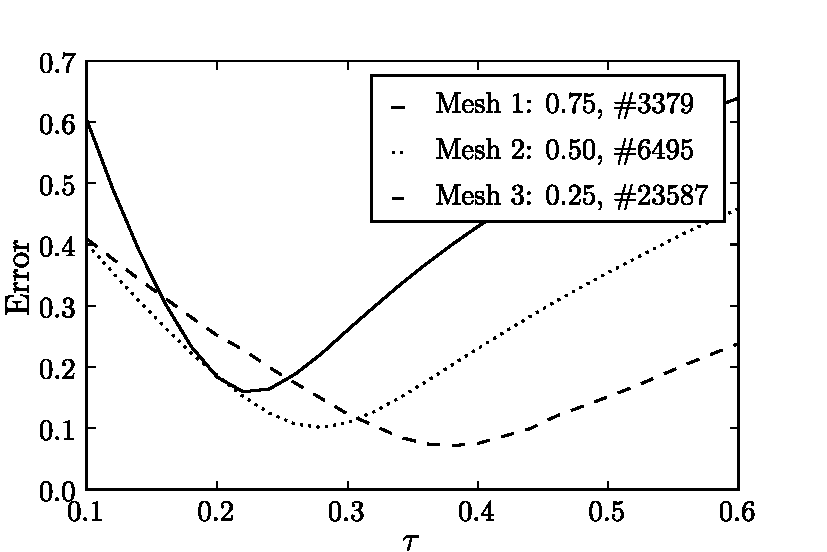
\includegraphics[width=\linewidth]{chapters/hake/pdf/error_plot}}
    \end{minipage}
    \hfill
    \begin{minipage}{\rightfigsize}
      \caption{The figure shows a plot of the error versus the stabilization parameter $\tau$ for 3 different mesh resolutions. The mesh resolutions are given by the median of the $z$ distance of all vertices and the total number of vertices in the mesh, see legend. We see that the minimal values of the error for the three meshes, occur at three different $\tau$: 0.22, 0.28, and 0.38.}
      \label{fig:error_plot}
    \end{minipage}
\end{figure}

\begin{figure}[b]
    \begin{minipage}[t]{\leftfigsize}
      \raisebox{-3.7cm}{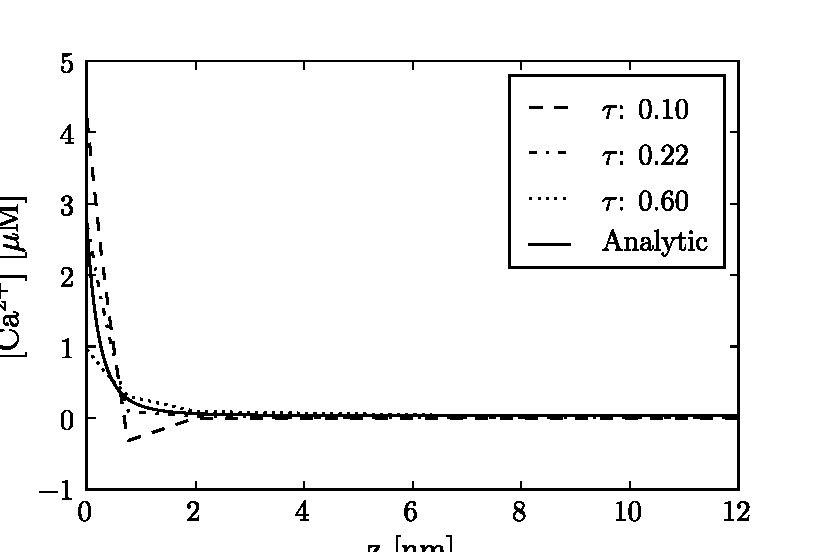
\includegraphics[width=\linewidth]{chapters/hake/pdf/traces_mesh_1}}
    \end{minipage}
    \hfill
    \begin{minipage}{\rightfigsize}
      \caption{The figure shows the concentration traces of the numerical solutions from Mesh 1, see legend of Fig.~\ref{fig:error_plot}, for three different $\tau$ together with the analytic solution. The solutions were picked from a line going between the points (0,0,0) and (0,0,12). We see that the solution with $\tau=0.10$ oscillates. The solution with $\tau=0.22$ was the solution with smallest global error for this mesh, see Fig~\ref{fig:error_plot}, and the solution with $\tau=0.60$ undershoots the analytic solution at $z=0$nm with \~1.7 $\mu$M.}
      \label{fig:traces_mesh_1}
    \end{minipage}
\end{figure}

The global stabilization parameter $\tau$, is problem dependent. To find an optimal $\tau$, for a certain electric field and mesh, the system in Eq.~(\ref{eq:algebraic-equation}) is solved to steady state, defined as T = 1.0 ms, using only homogeneous Neumann boundary conditions. An homogeneous concentration of $c_0=0.1$ $\mu$M is used as the initial condition. The numerical solution is then compared with the analytic solution of the problem. This solution is acquired by setting $J=0$ in Eq.~(\ref{eq:nernst-planck}) and solving for the $c$, with the following result:
\begin{equation}
  \label{eq:analytic-solution}
  c(z) = c_b\e^{-2\psi(z)}.
\end{equation}
Here $\psi$ is given by Eq.~(\ref{eq:electric_potential}), and $c_b$ is the concentration in the bulk, i.e., where $z$ is large. $c_b$ was chosen such that the integral of the analytic solution was equal to $c_0\times V$, where $V$ is the volume of the domain.\par

The error of the numerical solution for different values of $\tau$ and for three different mesh resolutions are plotted in Fig.~\ref{fig:error_plot}. The meshes are enumerated from 1-3. The error is computed using the L$^2(\Omega)$ norm and is normalized by the L$^2(\Omega)$ norm of the analytical solution,
\begin{equation}
  \label{eq:error_norm}
  \frac{\Ltwo{c(T)-c_h^{n_T}}}{\Ltwo{c(T)}},
\end{equation}
where $n_T$ is the time step at $t=T$. As expected, we see that the mesh with the finest resolution produces the smallest error. The mesh resolutions are quantified by the number of vertices close to $z=0$. In the legend of Fig.~\ref{fig:error_plot}, the median of the $z$ distance of all vertices and the total number of vertices in each mesh is presented. The three meshes were created such that the vertices closed to $z=0$ were forced to be situated at some fixed distances from $z=0$. Three numerical and one analytical solution for the three different meshes are plotted in Fig.~\ref{fig:traces_mesh_1}-~\ref{fig:traces_mesh_3}. The numerical solutions are from simulations using three different $\tau$: 0.1, 0.6 and the L$^2$-optimal $\tau$, see Fig.~\ref{fig:error_plot}. The traces in the figures are from the discrete solution $c_h^{n_T}$, evaluated on the straight line between the spatial points $p_0$=(0,0,0) and $p_1$=(0,0,12). \par

\newcommand{\captiontwo}{The figures show the concentration traces of the numerical solutions from Mesh 2, see legend of Fig.~\ref{fig:error_plot}, for three different $\tau$ together with the analytic solution. The solution traces in the two panels are picked from a line going between the spatial points (0,0,0) and (0,0,1.5), for the left panel, and between spatial points (0,0,10.5) and (0,0,12), for the right panel. We see from both panels that the solution with $\tau=0.10$ give the poorest solution. The solution with $\tau=0.28$ was the solution with smallest global error for this mesh, see Fig~\ref{fig:error_plot}, and this is reflected in the reasonable good fit seen in the left panel, especially at $z=0$nm. The solution with $\tau=0.60$ undershoots the analytic solution at $z=0$ with \~1.2 $\mu$M. From the right panel we see that all numerical solutions undershoot at $z=15$nm, and that the trace with $\tau=0.60$ comes the closest to the analytic solution.}

\begin{figure}[t]
  \centering
    \includegraphics[width=\leftfigsize]{chapters/hake/pdf/traces_mesh_2}
    \caption{\captiontwo}
    \label{fig:traces_mesh_2}
\end{figure}

\newcommand{\captionthree}{The figures shows the concentration traces of the numerical solutions from Mesh 3, see legend of Fig.~\ref{fig:error_plot}, for three different $\tau$ together with the analytic solution. The traces in the two panels were picked from the same lines as the one in Fig.~\ref{fig:traces_mesh_2}. Again we see from both panels that the solution with $\tau=0.10$ give the poorest solution. The solution with $\tau=0.38$ was the solution with smallest global error for this mesh, see Fig~\ref{fig:error_plot}, and this is reflected in the good fit seen in the left panel, especially at $z=0$nm. The solution with $\tau=0.60$ undershoots the analytic solution at $z=0$ with \~0.7 $\mu$M. From the right panel we see that all numerical solutions undershoot at $z=15$nm, and the trace with $\tau=0.60$ also here comes closest the analytic solution.}

\begin{figure}[t]
  \centering
    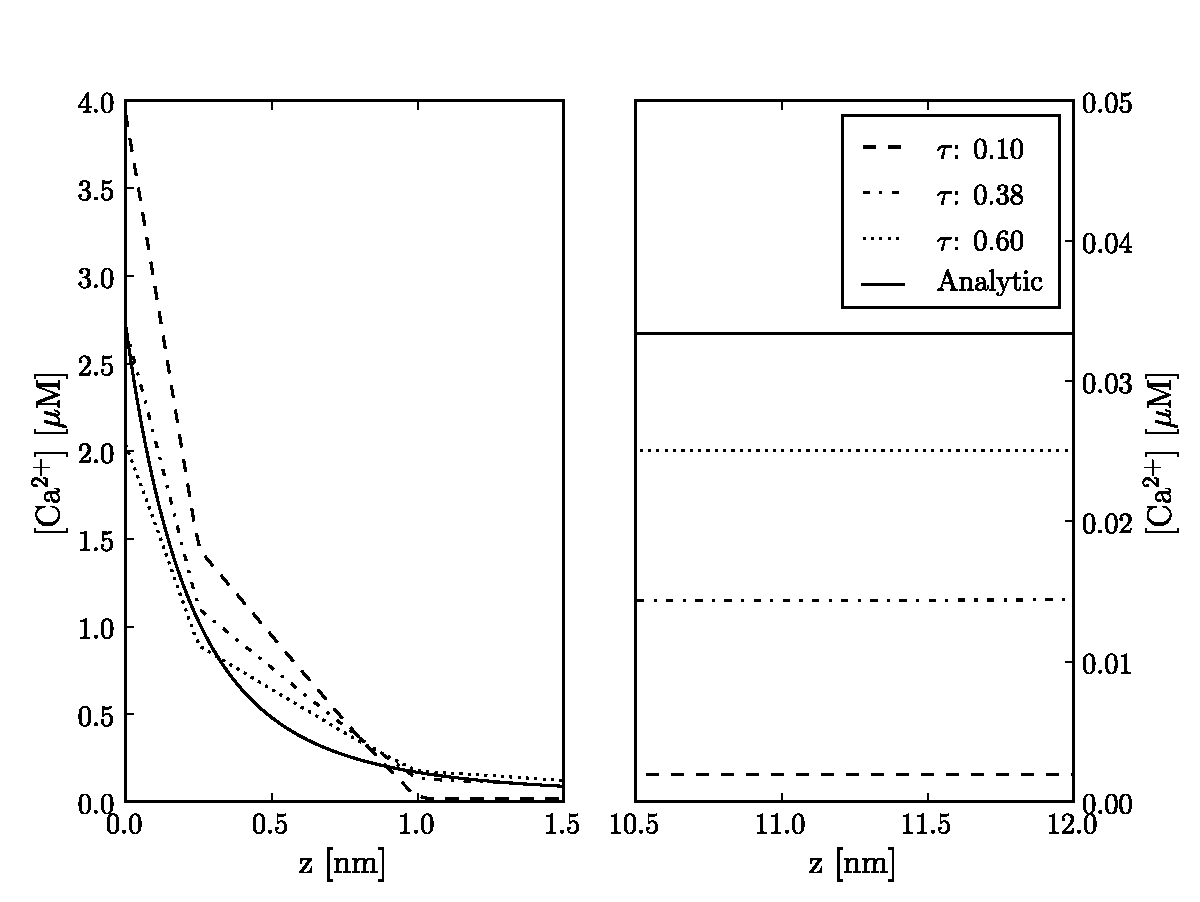
\includegraphics[width=\leftfigsize]{chapters/hake/pdf/traces_mesh_3}
    \caption{\captionthree}
    \label{fig:traces_mesh_3}
\end{figure}

In Fig.~\ref{fig:traces_mesh_1} the traces from mesh 1 is plotted. Here we see that the numerical solutions are quite poor for some of the $\tau$. The solution with $\tau=0.10$ is obviously not correct, as it produces negative concentrations. The solution with $\tau=0.60$ seems more correct but it undershoots the analytic solution at $z=0$ with \~ 1.7 $\mu$M. The solution with $\tau=0.22$ is the L$^2$-optimal solution for mesh 1, and approximates the analytic solution at $z=0$ well.\par

In Fig.~\ref{fig:traces_mesh_2} the traces from mesh 2 is presented in two plots. The left plot shows the traces for $z<1.5$ nm, and the right shows the traces for $z>10.5$ nm. In the left plot we see the same tendency as in Fig.~\ref{fig:traces_mesh_1}, an overshoot of the solution with $\tau=0.10$ and an undershoot of the solution with $\tau=0.60$. The L$^2$-optimal solution, the one with $\tau=0.28$, overshoots the analytic solution for the shown interval in the left plot, but undershoots for the rest of the trace. \par

In the last figure, Fig.~\ref{fig:traces_mesh_3}, traces from mesh 3 is presented. The results is also here presented in two plots, corresponding to the same $z$ interval as in Fig.~\ref{fig:traces_mesh_2}. We see that the solution with $\tau=0.10$ is not good in either plots. In the left plot it clearly overshoots the analytic solution for most of the interval, and then stays at a lower level than the analytic solution for the rest of the interval. The solution with $\tau=0.60$ is much better here than in the two previous plots. It undershoots the analytic solution at $z=0$ but stays closer to it for the rest of the interval than the L$^2$-optimal solution. The L$^2$ norm penalize larger distances between two traces, i.e., weighting the error close to $z=0$ more than the rest. The optimal solution measured in the Max norm is given when $\tau=50$, result not shown.\par

These results tell us that it is difficult to obtain accurate numerical solution for the advection-diffusion problem presented in Eq.~(\ref{eq:full_system}). Using a finer mesh close to $z=0$ could help, but it will create a larger algebraic system. It is interesting to notice that the L$^2$ optimal solutions is better close to $z=0$, than other solutions and the solution for the largest $\tau$ is better than other for $z$ > 2 nm. For a modeller, these constraints are important to know about; the solution at $z=0$ and $z=12$ nm are the most important, as \Ca interact with other proteins at these points.\par

\label{sec:solution}
\begin{figure}
  \centering
  \LVerbatimInput[fontsize=\scriptsize,frame=lines,
  framerule=0.4mm,
  xleftmargin=10mm,xrightmargin=15mm,
  numbers=left,numbersep=5pt]{chapters/hake/code/time_stepping_algorithm.py}
  \vspace{-1.5em}
  \caption{Python-like pseudo code for the time stepping algorithm used in our simulator}
  \label{fig:time-stepping-algorithm}
\end{figure}

\begin{figure}
  \centering
  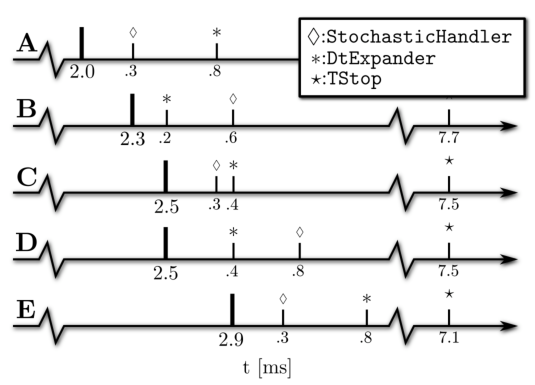
\includegraphics[width=0.6\linewidth]{chapters/hake/pdf/timeline}
  \caption{Diagram for the time stepping algorithm using 3 discrete objects: \texttt{DtExpander}, \texttt{StochasticHandler}, \texttt{TStop}. The values below the small ticks, corresponds to the time to the next event for each of the discrete objects. This time is measured from the last realized event, which is denoted by the thicker tick. In \textbf{A} we have realized a time event at t=2.0 ms. The next event to be realized is a stochastic transition, the one with smallest value below the ticks. In \textbf{B} this event is realized, and the \texttt{StochasticHandler} now show a new next event time. The event is a channel transition forcing the dt, controlled by the \texttt{DtExpander}, to be minimized. \texttt{DtExpander} now has the smallest next event time, and is realized in \textbf{C}. The channel transition that was realised in \textbf{B} raised the \CaC in the cleft which in turn increase the \Ca dependent propensity functions in the included Markov models. The time to next event time of the \texttt{StochasticHandler} has therefore been updated, and moved forward in \textbf{C}. Also note that the \texttt{DtExpander} has expanded its next event time. In \textbf{D} the stochastic transition is realized and updated with a new next event time, but it is ignored as it is not a channel transition. The smallest time step is now the \texttt{DtExpander}, and this is realized in \textbf{E}. In this example we do not realize the \texttt{TStop} event as it is too far away.}
  \label{fig:time-line}
\end{figure}

\section{\texttt{diffsim} an event driven simulator}
\label{sec:diffsim}
\index{time stepping}
\index{\texttt{diffsim}}
\index{FEniCS Apps}
In the scripts in Fig.~\ref{fig:assembly-algorithm}-~\ref{fig:solving-algorithm}, we show how a simple continuous solver can be built with \pydolfin. By preassembling the matrices from Eq.~(\ref{eq:matrices}) a flexible system for adding and removing boundary fluxes corresponding to the state of the channels can be constructed. The script in Fig.\ref{fig:solving-algorithm} uses fixed time points for the channel state transitions. At these time points we minimize \Dt, so we can resolve the sharp time gradient. In between the channel transitions we expand \Dt. This simplistic time stepping scheme is sufficient to solve the presented example. However it would be difficult to expand it to also incorporate the time stepping involved with the solution of stochastic Markov models, and other discrete variables. For such scenarios, an event driven simulator called \texttt{diffsim} has been developed. In the last subsections in this chapter, the algorithm underlying the time stepping scheme in \texttt{diffsim} will be presented. An example of how one can use \texttt{diffsim} to describe and solve a model of the \Ca dynamics in the dyadic cleft will also be demonstrated. The \texttt{diffsim} software can freely be downloaded from URL:\url{http://www.fenics.org/wiki/FEniCS_Apps}.\par

\subsection*{Stochastic system}
\label{sec:stochastic-system}
\index{Gillespie method}
\index{Markov chain model}
\index{propensity function}
\index{channel transition}
The stochastic evolution of the Markov chain models presented in Section \ref{sec:stochastic-models} is determined by a modified Gillespie method \cite{Gillespie1977}, which resembles the one presented in \citet{RudigerShuaiHuisingaEtAl2007}. Here we will not go into detail of the actual method, but rather explain the part of the method that has importance for the overall time stepping algorithm.\par

The solution of the included stochastic Markov chain models is stored in a state vector, \texttt{S}. Each element in \texttt{S} corresponds to one Markov model and the value reflects which state each model is in. The transitions between these states are modelled stochastically and are computed using the modified Gillespie method. This method basically gives us which of the states in \texttt{S} changes to what state and when. It is not all such state transitions that are relevant for the continuous system. A transition between two closed states in the LCC model will not have any impact on the boundary fluxes, and can be ignored. Only transitions that either open or close a channel (channel transitions), will be recognized. The modified Gillespie method assumes that any continuous variables that a certain propensity function depends on, are constant during a time step. The error of this assumption is reduced by taking smaller time steps right after a channel transition, as the continuous field is indeed changing dramatically during this time period. \par

\subsection*{Time stepping algorithm}
\label{sec:event-driven-simulator}
To simplify the presentation of the time stepping algorithm we only consider one continuous variable, this could for example be the \Ca field. The framework presented here can be expanded to also handle several continuous variables. We define a base class called \texttt{DiscreteObject}, which defines the interface for all discrete objects. A key function of a discrete object is to know when its \textit{next event} is due at. The \texttt{DiscreteObject} that has the smallest next event time, gets to define the size of the next \Dt. In \packagefont{Python} this is easily done by making the \texttt{DiscreteObject}s sortable with respect to their next event time. All \texttt{DiscreteObject}s is then collected in a list, \texttt{discrete\_objects} see Fig.~\ref{fig:time-stepping-algorithm}. The \texttt{DiscreteObject} with the smallest next event time is then just \texttt{min(discrete\_objects)}.\par

An event from a \texttt{DiscreteObject} that does not have an impact on the continuous solution will be ignored for example a Markov chain model transition that is not a channel transition. A transition needs to be realized before we can tell if it is a channel transition or not. This is done by \textit{stepping} the \texttt{DiscreteObject}, i.e., calling the object's \texttt{step()} method. If the method returns \texttt{False}, it will not affect the \Ca field, and we enter the while loop, and a new \texttt{DiscreteObject} is picked, see Fig.~\ref{fig:time-stepping-algorithm}. If the object returns \texttt{True} when stepped, we exit the loop and continue. Next, we have to update the other discrete objects with the chosen \Dt, solve for the \Ca field, broadcast the solution and last but not least execute the discrete event that is scheduled to happen at \Dt.\par

In Fig.~\ref{fig:time-line} we show an example of a possible realization of this algorithm. The example starts at t=2ms at the top-most timeline represented by \textbf{A}, and it includes three different types of \texttt{DiscreteObject}s: \texttt{i}) \texttt{DtExpander}, \texttt{ii}) \texttt{StochasticHandler}, and \texttt{iii}) \texttt{TStop}. See the figure legend for more details.\par
\begin{figure}
  \centering
  \LVerbatimInput[fontsize=\scriptsize,frame=lines,
  framerule=0.4mm,
  xleftmargin=10mm,xrightmargin=15mm,
  numbers=left,numbersep=5pt]{chapters/hake/code/diffsim_test.py}
  \vspace{-1.5em}
  \caption{An example of how \texttt{diffsim} can be used to simulate the time to RyR release latency, from a small dyad who's domain is defined by the mesh in the file \texttt{cleft\_mesh\_with\_RyR.xml.gz}.}
  \label{fig:diffsim_test}
\end{figure}

\subsection*{\texttt{diffsim}: an example}
\index{\texttt{diffsim}}
\index{event driven simulator}
\texttt{diffsim} is a versatile event driven simulator that incorporates the time stepping algorithm presented in the previous section together with the infrastructure to solve models with one or more diffusional domains, defined by a computational mesh. Each such domain can have several diffusive ligands. Custom fluxes can easily be included through the framework. The sub module \texttt{dyadiccleft} implements some published Markov models that can be used to simulate the stochastic behaviour of a dyad and some convenient boundary fluxes. It also implements the field flux from the lipid bi-layer discussed in Section~\ref{sec:ca-diffusion}. In Fig.~\ref{fig:diffsim_test} a runnable script is presented, which simulates the time to release, also called the latency, for a dyad. The two Markov models that is presented in Section \ref{sec:stochastic-models} are here used to model the stochastic dynamics of the RyRs and the LCCs. The simulation is driven by a so called dynamic voltage clamp. The data that defining the voltage clamp is read from a file using utilities from the \numpy \packagefont{Python} packages.\par

\section{Discussion}
We have presented a computational model of the \Ca dynamics of the dyadic cleft in heart cells. It consists of a coupled stochastic and continuous system. We have showed how one can use \pydolfin to discretise and solve the continuous system using a finite element method. The continuous system is an advection-diffusion equation that produce unstable discretizations. We investigate how one can use the streamline upwind/Petrov-Galerkin method to stabilize the discretized system. We use three different meshes and find an L$^2$-optimal global stabilization parameters $\tau$ for each mesh.\par

We do not present a solver for the stochastic system. However we outline a time stepping scheme that can be used to couple the stochastic solver with the presented solver for the continuous system. A simulator \texttt{diffsim} is briefly introduced, which implements the presented time stepping scheme together with the presented solver for the continuous system.
%\section{Introduction}
%\label{sec:intro}
%
%From when we are children we hear that we should drink milk because it is an important source for calcium (\Ca), and that \Ca is vital for a strong bone structure. What we do not hear as frequently, is that \Ca is one of the most important cellular messengers we have in our body \cite{Albe_2002_book}. Among other things \Ca controls cell death, neural signaling, secretion of different chemical substances to the body, and what will be our focus in this chapter, the contraction of cells in the heart.\par
%
%In this chapter I will first discribe a mathematical model that can be used to model \Ca dynamics in a small sub cellular domain called the dyadic cleft. The model includes \Ca diffusion that is described by an advection-diffusion partial differential equation, and discrete channel dynamics that is discribed by stochastic Markov models. Numerical methods implemented in \pydolfin solving the partial differental equation will also be presented. A time stepping scheme for solving the stochastic and deterministic models in a coupled manner will be presented in the last section. Here will also a solver framwork, \diffsim, that implements the time stepping scheme together with the other presented numerical methods be presented.\par
%
%\section{Biological background}
%\label{sec:morphology}
%In a healthy heart every beat origins in the sinusoidal node, where pacemaker cells triggers an electric signal. This signal propagates through the whole heart, and results in a sudden change in electric potential between the interior and exterior of the heart cells. These two domains are separated by the cell membrane. The difference in electric potential between these domains is called the membrane potential. The sudden change in the membrane potential, an action potential, is facilitated by specialized ion channels that reside in the membrane. When an action potential arrives a heart cell it triggers \Ca channel that brings \Ca into the cell. The \Ca then diffuse over a small cleft, called the dyadic cleft, and triggers further \Ca release from an intracellular \Ca storage, the sarcoplasmic reticulum (SR). The \Ca ions then diffuse to the main intracellular domain of the cell, the cytosole, in which the contractile proteins are situated. The \Ca ions attach to these proteins and triggers contraction. The strength of the contraction is controlled by the strength of the \Ca concentration in cytosole. The contraction is succeeded by a period of relaxation, which is facilitated by the extraction of \Ca from the intracellular space by various proteins. \par
%
%This chain of events is called the Excitation Contraction (EC) coupling \cite{Bers_2001_book}. Several severe heart diseases can be related to impaired EC coupling and by broaden the knowledge of the coupling it will also be possible to develop better treatments for the diseases. Although the big picture of EC coupling is straight forward to grasp it conceals the nonlinear action of hundreds of different protein species. Computational methods have emerged as a natural complement to experimental studies in the ongoing strive to better understand the intriguing coupling, and it is in this light the present study is presented. Here I will focus on the initial phase of the EC coupling, i.e., when \Ca flows into the cell and triggers further \Ca release.\par
%
%\begin{figure}[t]
%  \centering
%  \begin{minipage}{0.27\linewidth}
%    \fontfamily{cmss} \large \textbf{A}\\
%    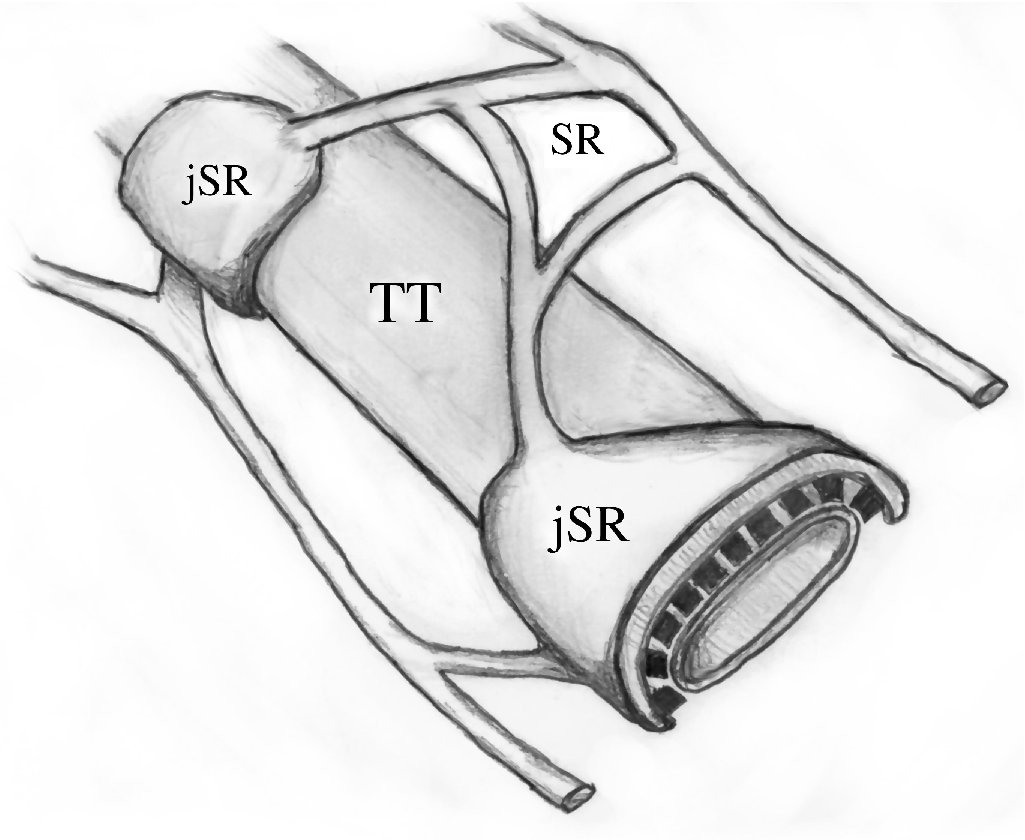
\includegraphics[width=\smallwidth]{chapters/hake/pdf/SR_TT.pdf}
%  \end{minipage}
%  \begin{minipage}{0.72\linewidth}
%    \fontfamily{cmss} \large \textbf{B}\\
%    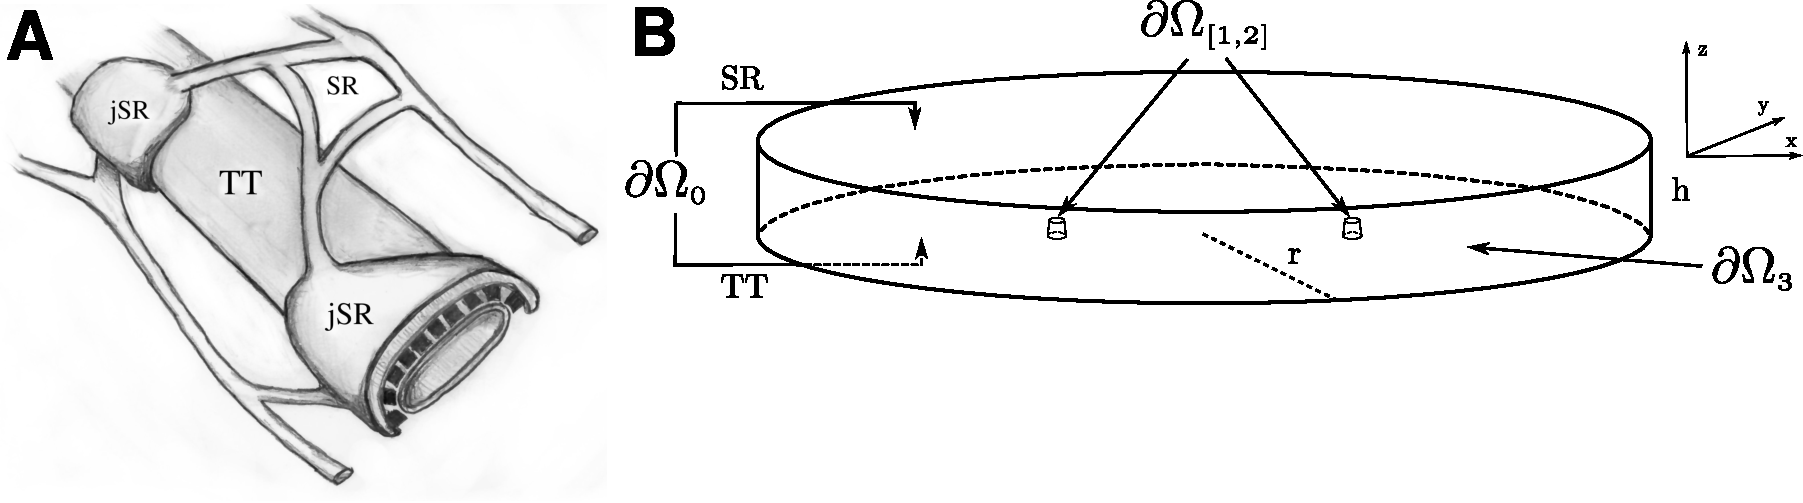
\includegraphics[width=\smallwidth]{chapters/hake/pdf/disk.pdf}
%  \end{minipage}
%  \caption{\textbf{A}: A diagram showing the relationship between the TT, the SR and the jSR. The volume between the flat jSR and the TT is the dyadic cleft. The black structures in the cleft are Ryanodine receptors, which are large channel proteins. The figure is from \cite{Broc_2005_3099}. \textbf{B}: The geometry that is used for the dyadic cleft. The top of the disk are the cell membrane of the SR, or jSR, the bottom the cell membrane of the TT, and the circumference of the disk is the interface to the cytosole. The top of the two small elevations models the mouths of two ion channels.}
%\label{fig:morphology}
%\end{figure}
%
%\section{Mathematical models}
%\label{sec:mathematical-models}
%%\think{Include an introduction of Mathematical models?}
%
%\subsection{Geometry}
%\label{sec:geometry}
%The dyadic cleft is the space between a structure called the t-tubule (TT) and the SR. TT is a network of pipe-like invaginations of the cell membrane that perforate the heart cell\cite{Soel_1999_266}. Fig.~\ref{fig:morphology} \textbf{A} presents a sketch of a small part of a single TT together with a piece of SR. Here one can see that the junctional SR (jSR) wraps the TT, and the small volume between these structures is the dyadic cleft. The space is not well defined as it is crowded with channel proteins, and the size of it also varies. In computational studies it is commonly approximated as a disk or a rectangular slab \cite{Pesk_1992_59,SoellerCannel1997,Koh_2006_1999,Tans_2007_3379}. In this study I have used a disk, see Fig.~\ref{fig:morphology} \textbf{A}. The height of the disk is: $h = 12$nm, and the radius is: $r = 50$nm. Larger radius can be used, e.g., up to 200 nm, but due to numerical limitations I have to limit the size of the cleft, see below. The diffusion constant of \Ca was set to $\sigma$ = $10^5$ nm$^2$ ms$^{-1}$ \cite{Lang_1996_1169}.\par
%
%\subsection{\Ca Diffusion}
%\label{sec:ca-diffusion}
%%\think{Include an introduction of \Ca diffusion?}
%
%\paragraph{Electro-Diffusion}
%The cell membrane, also called the sarcolemma, consists of a lipid bi-layer, which produce an electric potential in the solution. This potential is due to negatively charged phospholipid head-groups \cite{McLa_1971_667,Lang_1990_335}. Therefore in close proximity to the sarcolemma, an electric double layer is produced \cite{Bard_2001_book}. I am going to use the Gouy-Chapman method, which defines a \textit{diffuse layer} to describe this double layer \cite{Grah_1947_441}. The theory introduces an advection term to the ordinary diffusion equation, which makes the resulting equation harder to solve. \par
%
%The ion flux in a solution that experience an electric field is governed by the Nernst-Planck equation,
%\begin{equation}
%  \label{eq:nernst-planck}
%  J = -\sigma\left(\nabla c-2\,cE\right),
%\end{equation}
%where $\sigma$ is the diffusion constant of \Ca, $c = c(x,t)$ is the \Ca concentration, $E = E(x)$ is the non-dimensional electric field (the original electric field scaled with $e/kT$) and 2 is the valence of \Ca. Assuming conservation of mass, we arrive at the general advection-diffusion equation,
%\begin{equation}
%  \label{eq:advection-diffusion}
%  \dot{c}=\sigma\left[\Delta c - \nabla\cdot\left(2\,cE\right)\right].
%\end{equation}
%$E$ follows from the non-dimensional potential, $\psi$, (the ordinary electric potential scaled with e/kT) in the solution as,
%\begin{equation}
%  \label{eq:electric_field}
%  E=-\nabla\psi.
%\end{equation}
%The strength of $\psi$ is defined by the amount of charged head-groups in the lipid bi-layers and by the combined screening effect of all ions in the dyadic cleft. Following previous work done by \cite{Lang_1990_335} and \cite{SoellerCannel1997} all other ions in the solution will be treated as being in steady state. The sarcolemma is assumed to be planar and effectively infinite. This let us use an approximation of the electric potential in the solution,
%\begin{equation}
%  \label{eq:electric_potential} \psi(z) = \psi_0\exp(-\kappa{}z).
%\end{equation}
%Here $\psi_0$ is the non-dimensional potential at the membrane, $\kappa$ the inverse Debye length and $z$ the distance from the sarcolemmar in a perpendicular direction. \cite{SoellerCannel1997} showed that for a large range of \CaC, $\psi_0$ stayed constant at -2.2 and $\kappa$ is also assumed to be 1 nm. \par
%
%\editornote{Check formula in (\ref{eq:electric_potential}). Got undefined control sequence when comping
%so needed to edit.}
%
%\paragraph{Boundary fluxes}
%The SR and TT membrane is impermeable for ions, effectively making $\partial\Omega_{\scriptscriptstyle\text{0}}$, in Fig.~\ref{fig:morphology}, a no-flux boundary, giving us,
%\begin{equation}
%  \label{eq:no-flux}
%  J_{\scriptscriptstyle 0}= 0.
%\end{equation}
%The main sources for \Ca inflow to the dyadic cleft in our model, is the L-type \Ca channel (LCC). This flux comes in at the $\partial\Omega_{\scriptscriptstyle\text{[1,2]}}$ boundaries, see Fig.~\ref{fig:morphology}. After entering the cleft the \Ca then diffuse to the RyR situated at the SR membrane, triggering more \Ca influx. This flux will not be included in the simulations, however the stochastic dynamic of the opening of the channel will be included, see Section \ref{sec:stochastic-models} below. The \Ca that enters the dyadic cleft diffuse into the main compartement of cytosole introducing a third flux at the $\partial\Omega_{\scriptscriptstyle\text{3}}$ boundary.\par
%
%The LCC is a stochastic channel that are modelled as either open or close. When the channel is open \Ca flows into the cleft. The dynamic that describes the stochastic behaviour is presented in Section \ref{sec:stochastic-models} below. The LCC flux is modelled as a constant current with amplitude, -0.1 pA, which corresponds to the amplitude during voltage clamp to 0 mV \cite{Guia_2001_2742}. The LCC flux is then,
%%or as a Voltage and \CaC dependent current, using the constant field approximation \cite{Luo_1994_1071,Camp_1988_267}. The first flux is given by,
%\begin{equation}
%\label{eq:constant-current-flux}
%J_{\scriptscriptstyle[1,2]}= \left\{
%  \begin{array}{c@{\quad:\quad}l}
%    0& \text{close channel}\\
%    - \frac{i}{2\,F\,A},& \text{open channel}
%  \end{array}
%\right.
%\end{equation}
%\noindent where $i$ is the amplitude, 2 the valence of \Ca, $F$ Faraday's constant and $A$ the area of the channel. Note that inward current is by convention negative.\par
%
%\editornote{Placement of figures seems strange.}
%
%The flux to cytosole is modeled as a concentration dependent flux,
%\begin{equation}
%  \label{eq:conc-dependent-flux}
%  J_{\scriptscriptstyle 3}= -\sigma\frac{c - c_0}\Ds,
%\end{equation}
%where $c$ is the concentration in the cleft at the boundary, $c_0$ the concentration in cytosole, and \Ds the distance to the center of the cytosole.\par
%
%\begin{figure}[t]
%  \centering
%  \begin{minipage}{0.79\linewidth}
%    \fontfamily{cmss} \large \textbf{A}\\[0.5em]
%    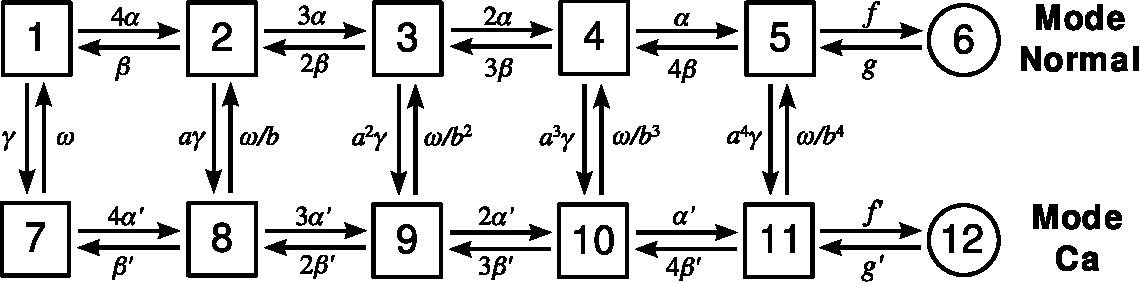
\includegraphics[width=\smallwidth]{chapters/hake/pdf/Jafri_1998_LCC_model.pdf}
%  \end{minipage}
%  \begin{minipage}{0.2\linewidth}
%    \fontfamily{cmss} \large \textbf{B}\\[0.5em]
%    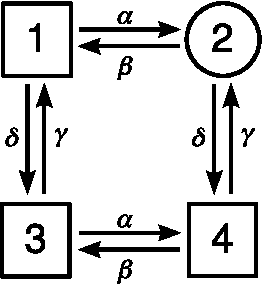
\includegraphics[width=\smallwidth]{chapters/hake/pdf/Stern_1999_RyR_model.pdf}
%  \end{minipage}
%\caption{\textbf{A}: State diagram of the discrete LCC Markov model from \cite{JafriRiceWinslow1998}. Each channel can be in one of the 12 states.  The transition between the states are controlled by propensities. The $\alpha$, and $\beta$ are voltage dependent, $\gamma$ is \CaC dependent and $f$, $a$, $b$, and $\omega$ are constant, see \cite{JafriRiceWinslow1998} for further details. The channels operates in two modes: \textit{Mode normal}, represented by the states in the upper row, and \textit{Mode Ca}, represented the states in the lower row. In state 6 and 12 the channel is open, but state 12 is rarely entered as $f'\ll{}f$, effectively making \textit{Mode Ca} an inactivated mode.
%\textbf{B}: State diagram of a RyR from \cite{Ster_1999_469}. The $\alpha$ and $\gamma$ propensities are \Ca dependent, representing the activation and inactivation dependency of the cytosolic \CaC. The $\beta$ and $\delta$ propensities are constant.}
%\label{fig:markov-models}
%\end{figure}
%
%\subsection{Stochastic models of single channels}
%\label{sec:stochastic-models}
%Discrete and stochastic Markov chain models are used to describe single channels dynamics. Such models consists of a variable that can be in a certain number of discrete states. The transition between these states is a stochastic event. The frequency of these events are determined by the propensity functions associated to each transition. These functions characterize the probability per unit time that the corresponding transition event occurs and are dependent on the chosen Markov chain model and they may vary with time.\par
%
%\paragraph{L-type \Ca channel}
%\label{sec:lcc}
%The LCC is the main source for extracellular \Ca into the cleft. The channel opens when an action potential arrives to the cell and inactivates when single \Ca ions binds to binding sites on the intracellular side of the channel. An LCC is composed by a complex of four transmembrane subunits, which each can be permissive or non-permissive. For the whole channel to be open, all four subunits need to be permissive and the channel then has to undergo a last conformational change to an opened state \cite{Hill_2001_book}. In this chapter I am going to use a Markov model of the LCC that incorporates a voltage dependent activation together with a \Ca dependent inactivation \cite{JafriRiceWinslow1998,Gree_2002_2918}. The state diagram of this model is presented in Fig.~\ref{fig:markov-models} \textbf{A}. It consists of 12 states, where state 6 and 12 are the only conducting states, i.e., when the channel is in one of these states it is open. The transition propensities are defined by a set of functions and constants, which are all described in \cite{Gree_2002_2918}.\par
%
%\paragraph{Ryanodine Receptors}
%\label{sec:ryr}
%RyRs are \Ca specific channels that are situated on the SR in clusters of several channels \cite{Beuc_1988_233,Fran_1999_1528}. They open by single \Ca ions attaching to the receptors at the cytosolic side. A modified version of a phenomenological model that mimics the physiological functions of the RyRs, first presented by \cite{Ster_1999_469}, will be used. The model consists of four states where one is conducting, state 2, see Fig.~\ref{fig:markov-models} \textbf{B}. The $\alpha$ and $\gamma$ propensities are \Ca dependent, representing the activation and inactivation dependency of cytosolic \CaC. The $\beta$ and $\delta$ propensities are constants. For specific values for the propensities consider \cite{Ster_1999_469}.\par
%
%\section{Numerical methods for the continuous system}
%The continuous problem is defined by Eq.~(\ref{eq:advection-diffusion}~-\ref{eq:conc-dependent-flux}) together with an initial condition. Given a bounded domain $\Omega \subset \Rset^3$ with the boundary, $\partial\Omega$, we want to find $c = c(x,t) \in \Rset_+$, for $x\in \Omega$ and $t \in \Rset_+$, such that:
%\begin{equation}
%%\renewcommand{\arraystretch}{1.5}
%%\renewcommand{\baselinestretch}{1.5}
%\label{eq:full_system}
%\left\{
%  \begin{array}{r@{\quad=\quad}ll}
%    \dot{c}&\sigma\Delta c - \nabla\cdot\left(ca\right)&  \text{in } \Omega \\
%    \sigma\diff[c]{n}&J_k& \text{on } \partial\Omega_k,
%  \end{array}
%\right.
%%\renewcommand{\arraystretch}{1}
%%\renewcommand{\baselinestretch}{1}
%\end{equation}
%with $c(\cdot,0) = c_0(x)$. Here $a=a(x)=2\sigma E(x)$, and, $J_k$ and $\partial\Omega_k$ are the \kth flux at the \kth boundary, where $\bigcup_k\partial\Omega_k=\partial\Omega$. The $J_k$ are given by Eq.~(\ref{eq:no-flux})-~(\ref{eq:conc-dependent-flux}).\par
%
%\begin{figure}
%  \centering
%  \LVerbatimInput[fontsize=\scriptsize,frame=lines,
%  framerule=0.4mm,
%  xleftmargin=10mm,xrightmargin=15mm,
%    numbers=left,numbersep=5pt]{chapters/hake/code/matrix_assemble.py}
%  \vspace{-1.5em}
%  \caption{Python code for the assembly of the matrices and vectors from Eq.~(\ref{eq:matrices})-(\ref{eq:vector}).}
%  \label{fig:assembly-algorithm}
%\end{figure}
%
%\subsection{Discretization}
%\label{sec:discretization}
%The continuous equations are discretized using the Finite element method. Eq.~(\ref{eq:full_system}) is multiplied with a proper test function, $v$, and we get:
%\begin{equation}
%  \label{eq:advection-diffusion-weak-form-0}
%  \int_\Omega\dot{c}v\,dx = \int_\Omega \left[\sigma\Delta c-\nabla(ca)\right] v\,dx,
%\end{equation}
%and we integrate by part and get:
%\begin{equation}
%  \label{eq:advection-diffusion-weak-form}
%  \int_\Omega\dot{c}v\,dx = -\int_\Omega \left(\sigma\nabla c-ca\right)\nabla v\,dx + \sum_k\int_{\partial\Omega_k} J_kv\,ds_k.
%\end{equation}
%Consider a tetrahedralization of $\Omega$, a mesh, where the domain is divided into disjoint subdomains, $\Omega_e$, elements. A discrete solution $c_h\in V_h$ is defined. Here $V_h=\{ \phi \in H^1(\Omega):\phi\in P^k(\Omega_e)\forall e\}$, and $P^k$ represents the space of Lagrange polynomials of order $k$. The backward Euler method is used to approximate the time derivative and Eq.~(\ref{eq:advection-diffusion-weak-form}) can now be stated as follows: given $c_h^n$ find $c_h^{n+1} \in V_h$ such that:
%\begin{equation}
%  \label{eq:advection-diffusion-weak-discrete-form}
%  \int_{\Omega} \frac{c_h^{n+1}-c_h^{n}}{\Dt}v\,dx = -\int_{\Omega} \left(\sigma\nabla c_h^{n+1}-c_h^{n+1}a\right)\cdot\nabla v\,dx + \sum_k\int_{\partial\Omega} J_kv\,ds_{k},\forall v \in V_h
%\end{equation}
%where \Dt is the time step. The trial function $c^n_h(x)$ is expressed as a weighted sum of basis functions,
%\begin{equation}
%  \label{eq:discrete-solution}
%  c^n_h(x) = \sum^N_j C_j^n\phi_j(x),
%\end{equation}
%where $C_j^n$ are the coefficients. Lagrange polynomials of first order is used for both the test and the trial function, $k=1$, and the number of unknowns, $N$, will then coincide with the number of vertices of the mesh.\par
%
%\begin{figure}
%  \centering
%  \LVerbatimInput[fontsize=\scriptsize,frame=lines,
%  framerule=0.4mm,
%  xleftmargin=10mm,xrightmargin=15mm,
%  numbers=left,numbersep=5pt]{chapters/hake/code/stabilization.py}
%  \vspace{-1.5em}
%  \caption{Python code for the assembly of the SUPG term for the mass and advection matrices.}
%  \label{fig:SUPG-assembly-algorithm}
%\end{figure}
%The test function $v$ is chosen from the same discrete basis as $c^n_h(x)$, i.e., $v_i(x) = \phi_i(x)\in V_h$, for $i \in [1\ldots N]$. These are used in Eq.~(\ref{eq:advection-diffusion-weak-discrete-form}) to produce an algebraic problem on the following form:
%\begin{equation}
%  \label{eq:algebraic-equation}
%  \frac{1}{\Dt}\text{\bfseries\itshape M}\left(C^{n+1}-C^n\right) =  \left(-\text{\bfseries\itshape K}+\text{\bfseries\itshape E}+\sum_k\alpha^k\text{\bfseries\itshape F}^k\right)C_j^{n+\frac{1}{2}}+\sum_k c_0^k\,f^k,
%\end{equation}
%where $C^n\in \Rset^N$ is the vector of coefficients from the discrete solution $c^n_h(x)$, $\alpha^k$ and $c_0^k$ are constant coefficients related to the \kth flux and\\[-1.0em]
%\begin{equation}
%  \renewcommand{\arraystretch}{1.7}
%  \renewcommand{\baselinestretch}{1.7}
%  \begin{array}{r@{\;=\;}lcr@{\;=\;}l}
%    M_{ij}&\displaystyle\int_\Omega\phi_i\phi_jdx,& \quad\quad&K_{ij}&\displaystyle\int_\Omega\nabla\phi_i\cdot\nabla\phi_jdx,\\
%    E_{ij}&\displaystyle\int_\Omega a\phi_i\cdot\nabla\phi_jdx,& \quad\quad&F^k_{ij}&\displaystyle\int_{\partial\Omega_k}\phi_i\phi_jds,
%  \end{array}
%  \renewcommand{\arraystretch}{1}
%  \renewcommand{\baselinestretch}{1}
%  \label{eq:matrices}
%\end{equation}
%are the entries in the {\bfseries\itshape M}, {\bfseries\itshape K}, {\bfseries\itshape E} and {\bfseries\itshape F}$^k$ matrices. $f^k$ are boundary source vectors corresponding to the \kth boundary. The vector elements are given by:
%\begin{equation}
%  \label{eq:vector}
%  f^k_{i}=\int_{\partial\Omega_k}\phi_ids.
%\end{equation}
%%Note that $a$ is a function given by a finite element vector space. In Section \ref{sec:results} we will show the impact different orders of this space has on the final result.\par
%
%The code for producing the matrices and vectors in Eq.~(\ref{eq:matrices})-(\ref{eq:vector}) is presented in Fig. \ref{fig:assembly-algorithm}. Note that in the last for loop we iterate over the unique subdomains, and set the entries of the \texttt{MeshFunction} \texttt{domain} corresponding to the \kth boundary to 0 and the other entries to 1. In this way the same form for the exterior facet domain integrals can be used.\par
%
%The system in Eq.~(\ref{eq:algebraic-equation}) is linear and the matrices and vectors can be pre-assembled. This allows for a flexible system where boundary matrices and boundary source vectors can be added, when a channel opens. \Dt can also straightforwardly be decreased when such an event occurs. This adaptation in time is crucial both for the numerical stability of the linear system. \Dt can then be increased after each time step as the demand on the size of \Dt falls. The sparse linear system is solved using the \petsc linear algebra backend\cite{www:petsc} in \pydolfin together with the Bi-CGSTAB iterative solver \cite{Vors_1992_631}, and the BoomerAMG preconditioners from hypre\cite{Falg_2002_632_inproc}. In Fig.~\ref{fig:solving-algorithm} a script is presented that solves the algebraic system from Eq.~(\ref{eq:algebraic-equation}) together with a crude time stepping scheme for the opening and closing of the included LCC flux.\par
%
%\subsection{Stabilization}
%\label{sec:stabilization}
%It turns out that the algebraic system in Eq.~(\ref{eq:algebraic-equation}) is numerically unstable for physiological relevant values of $a$, see Section \ref{sec:ca-diffusion}. This is due to the transport term introduced by $A_{ij}$ from Eq.~(\ref{eq:matrices}). I have chosen to stabilize the system using the Streamline upwind Petrov-Galerkin (SUPG) method \cite{Broo_1982_199}. This method adds a discontinuous streamline upwind contribution to the testfunction in Eq.~(\ref{eq:advection-diffusion-weak-form-0}),
%\begin{equation}
%  \label{eq:stabilizing-term}
%  v' = v+s, \text{ where } s = \tau\frac{h\tau_l}{2\|a\|}a\cdot\nabla v.
%\end{equation}
%Here $\tau\in[0,1]$ is problem dependent, $h=h(x)$ is the size of the local element of the mesh, and $\tau_l=\tau_l(x)$, is given by,
%\begin{equation}
%  \label{eq:local-tau}
%  \tau_l=\coth(\PEl)-1/\PEl,
%\end{equation}
%where $\PEl$ is the local P\'eclet number:
%\begin{equation}
%  \label{eq:peclet}
%  \PEl = \|a\|h/2\sigma.
%\end{equation}
%This form of $\tau_l$ follows the optimal stabilization from an 1D case\cite{Broo_1982_199}, other choices exist. The contribution from the diffusion term of the weak form can be eliminated by choosing a test function from a first order Lagrange polynomial, as the $\Delta$ operator will reduce the trial function to zero. The \pydolfin code that assembles the SUPG part of the problem is presented in Fig.~\ref{fig:SUPG-assembly-algorithm}. In the script two matrices, \texttt{E\_stab} and \texttt{M\_stab} are assembled, which are both added to the corresponding advection and mass matrices \texttt{E} and \texttt{M} weighted by the global parameter \texttt{tau}.\par
%
%A mesh with finer resolution close to the TT surface, at $z=0$ nm, is also used to further increase the stability. It is at this point the electric field is at its strongest and it attenuates fast. At $z=3$ nm the field is down to 5\% of the maximal amplitude, and at $z=5$ nm, it is down to 0.7\%, reducing the need for high mesh resolutions. The mesh generator \texttt{tetgen} is used to to produce meshes with the needed resolution \cite{www:tetgen}.\par
%
%\begin{figure}
%  \centering
%  \LVerbatimInput[fontsize=\scriptsize,frame=lines,
%  framerule=0.4mm,
%  xleftmargin=10mm,xrightmargin=15mm,
%  numbers=left,numbersep=5pt]{chapters/hake/code/solving.py}
%  \vspace{-1.5em}
%  \caption{Python code for solving the system in Eq.~(\ref{eq:algebraic-equation}), using the assembled matrices from the two former code examples from Fig.~\ref{fig:assembly-algorithm}-~\ref{fig:SUPG-assembly-algorithm}.}
%  \label{fig:solving-algorithm}
%\end{figure}
%
%\newcommand{\leftfigsize}{0.66\linewidth}
%\newcommand{\rightfigsize}{0.31\linewidth}
%
%\begin{figure}[t]
%    \begin{minipage}[t]{\leftfigsize}
%      \raisebox{-3.45cm}{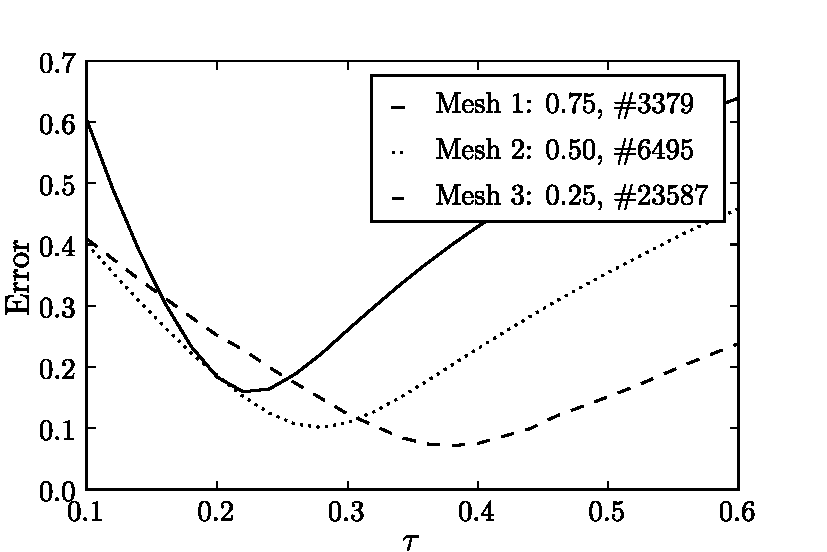
\includegraphics[width=\largewidth]{chapters/hake/pdf/error_plot.pdf}}
%    \end{minipage}
%    \hfill
%    \begin{minipage}{\rightfigsize}
%      \caption{The figure shows a plot of the error (a normalized L2 norm of the difference between the numerical and analytical solutions) against the stabilization parameter $\tau$ for 3 different mesh resolutions. The mesh resolutions are given by the median of the $z$ distance of all vertices and the total number of vertices in the mesh, see legend. We see that the minimal values of the error for the three meshes, occur at three different $\tau$: 0.22, 0.28, and 0.38.}
%      \label{fig:error_plot}
%    \end{minipage}
%\end{figure}
%
%\begin{figure}[b]
%    \begin{minipage}[t]{\leftfigsize}
%      \raisebox{-3.7cm}{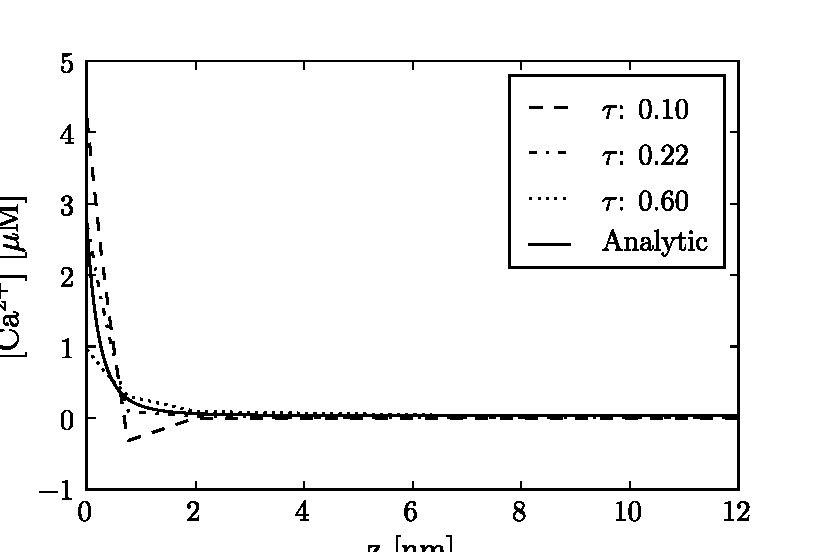
\includegraphics[width=\largewidth]{chapters/hake/pdf/traces_mesh_1.pdf}}
%    \end{minipage}
%    \hfill
%    \begin{minipage}{\rightfigsize}
%      \caption{The figure shows the concentration traces of the numerical solutions from Mesh 1, see legend of Fig.~\ref{fig:error_plot}, for three different $\tau$ together with the analytic solution. The solutions were picked from a line going between the points (0,0,0) and (0,0,12). We see that the solution with $\tau=0.10$ oscillates. The solution with $\tau=0.22$ was the solution with smallest global error for this mesh, see Fig~\ref{fig:error_plot}, and the solution with $\tau=0.60$ undershoots the analytic solution at $z=0$nm with \~1.7 $\mu$M.}
%      \label{fig:traces_mesh_1}
%    \end{minipage}
%\end{figure}
%
%The global stabilization parameter $\tau$, is problem dependent. To find an optimal $\tau$, for a certain electrical field and mesh, the sytem in Eq.~(\ref{eq:algebraic-equation}) is solved to steady state using only homogeneous Neumann boundary conditions. An homogeneous concentration of $c_0=0.1$ $\mu$M is used as the initial condition. The numerical solution is then compared with the analytic solution of the problem. This solution is acquired by setting $J=0$ in Eq.~(\ref{eq:nernst-planck}) and solving for the $c$, with the following result:
%\begin{equation}
%  \label{eq:analytic-solution}
%  c(z) = c_b\exp(-2\psi(z)).
%\end{equation}
%Here $\psi$ is given by Eq.~(\ref{eq:electric_potential}), and $c_b$ is the concentration in the bulk, i.e., where $z$ is large. $c_b$ was chosen such that the integral of the analytic solution was equal to $c_0\times V$, where $V$ is the volume of the domain.\par
%
%\editornote{Check equation (\ref{eq:analytic-solution}).}
%
%The error of the numerical solution for different values of $\tau$ and for three different mesh resolutions are plotted in Fig.~\ref{fig:error_plot}. The meshes are enumerated from 1-3. The error is given in a normalized L2 norm. As expected we see that the mesh with the finest resolution produce the smallest error. The mesh resolutions are quantified by the number of vertices close to $z=0$. In the legend of Fig.~\ref{fig:error_plot} the median of the $z$ distance of all vertices and the total number of vertices in each mesh is presented. The three meshes were created such that the vertices closed to $z=0$ were forced to be situated at some fixed distances from $z=0$. Three numerical and one analytical solution for the three different meshes are plotted in Fig.~\ref{fig:traces_mesh_1}-~\ref{fig:traces_mesh_3}. The numerical solutions are from simulations using three different $\tau$: 0.1, 0.6 and the L2-optimal $\tau$, see Fig.~\ref{fig:error_plot}. The traces in the figures are all picked from a line going from (0,0,0) to (0,0,12). \par
%
%\newcommand{\captiontwo}{The figures shows the concentration traces of the numerical solutions from Mesh 2, see legend of Fig.~\ref{fig:error_plot}, for three different $\tau$ together with the analytic solution. The traces in the two panels were picked from a line going between the points (0,0,0) and (0,0,1.5) for the left panel and between (0,0,10.5) and (0,0,12) for the right panel. We see from both panels that the solution with $\tau=0.10$ give the poorest solution. The solution with $\tau=0.28$ was the solution with smallest global error for this mesh, see Fig~\ref{fig:error_plot}, and this is reflected in the reasonable good fit seen in the left panel, especially at $z=0$nm. The solution with $\tau=0.60$ undershoots the analytic solution at $z=0$ with \~1.2 $\mu$M. From the right panel we see that all numerical solutions undershoot at $z=15$nm, and that the trace with $\tau=0.60$ comes closest the analytic solution.}
%%\begin{figure}[t]
%%    \begin{minipage}[t]{\leftfigsize}
%%      \raisebox{-4cm}{\includegraphics[width=\linewidth]{traces_mesh_2}}
%%    \end{minipage}
%%    \hfill
%%    \begin{minipage}{\rightfigsize}
%%      \caption{\captiontwo}
%%      \label{fig:traces_mesh_2}
%%    \end{minipage}
%%\end{figure}
%
%\begin{figure}[t]
%  \centering
%    \includegraphics[width=\leftfigsize]{chapters/hake/pdf/traces_mesh_2.pdf}
%    \caption{\captiontwo}
%    \label{fig:traces_mesh_2}
%\end{figure}
%
%\newcommand{\captionthree}{The figures shows the concentration traces of the numerical solutions from Mesh 3, see legend of Fig.~\ref{fig:error_plot}, for three different $\tau$ together with the analytic solution. The traces in the two panels were picked from the same lines as the one in Fig.~\ref{fig:traces_mesh_2}. Again we see from both panels that the solution with $\tau=0.10$ give the poorest solution. The solution with $\tau=0.38$ was the solution with smallest global error for this mesh, see Fig~\ref{fig:error_plot}, and this is reflected in the good fit seen in the left panel, especially at $z=0$nm. The solution with $\tau=0.60$ undershoots the analytic solution at $z=0$ with \~0.7 $\mu$M. From the right panel we see that all numerical solutions undershoot at $z=15$nm, and the trace with $\tau=0.60$ also here comes closest the analytic solution.}
%
%\begin{figure}[t]
%  \centering
%    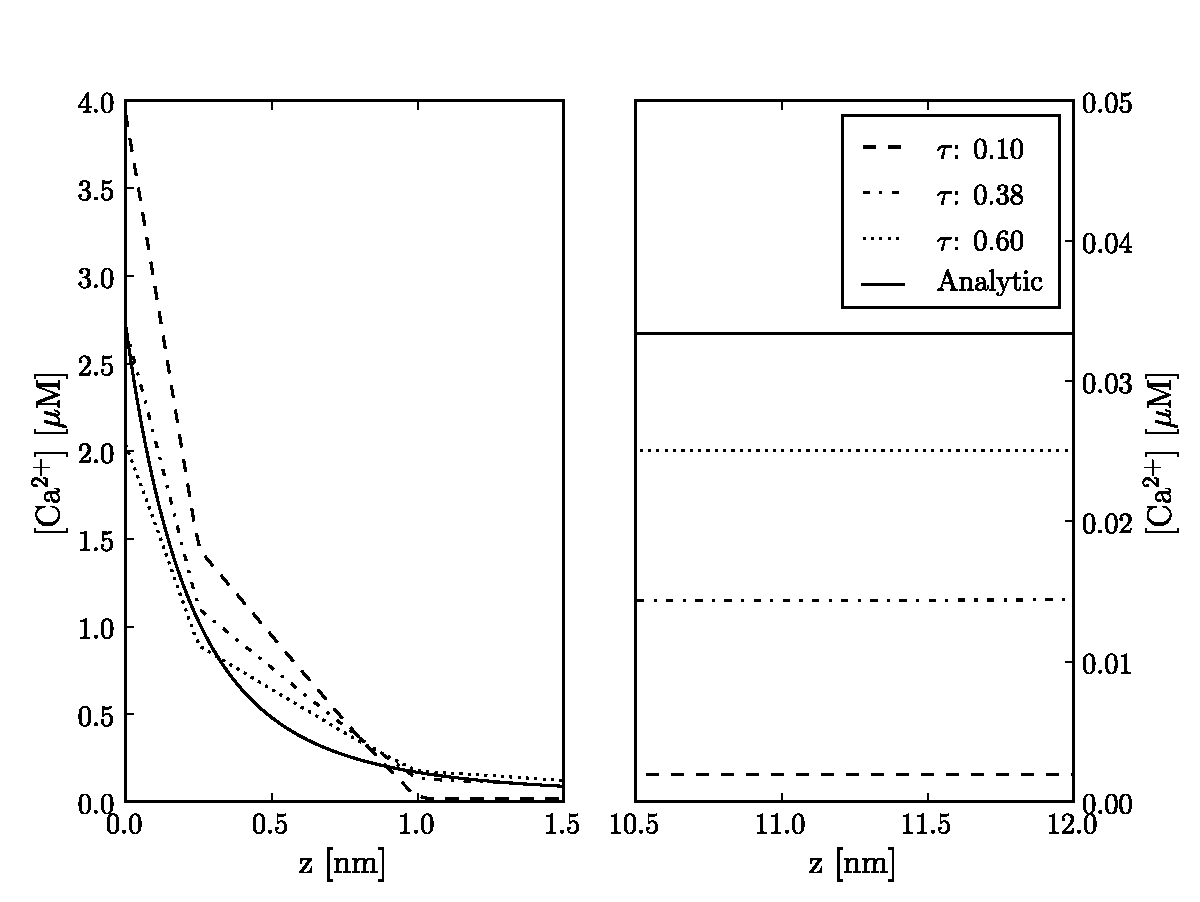
\includegraphics[width=\leftfigsize]{chapters/hake/pdf/traces_mesh_3.pdf}
%    \caption{\captionthree}
%    \label{fig:traces_mesh_3}
%\end{figure}
%
%In Fig.~\ref{fig:traces_mesh_1} the traces from mesh 1 is plotted. Here we see that all numerical solutions are quite poor for all $\tau$. The solution with $\tau=0.10$ is unstable as it oscillates and produces negative concentration. The solution with $\tau=0.60$ seems stable but it undershoots the analytic solution at $z=0$ with \~ 1.7 $\mu$M. The solution with $\tau=0.22$ is the L2-optimal solution for mesh 1, and approximates the analytic solution at $z=0$ well.\par
%
%In Fig.~\ref{fig:traces_mesh_2} the traces from mesh 2 is presented in two plots. The left plot shows the traces for $z<1.5$ nm and the right shows the traces for $z>10.5$ nm. In the left plot we see the same tendency as in Fig.~\ref{fig:traces_mesh_1}, an overshoot of the solution with $\tau=0.10$ and an undershoot for the solution with $\tau=0.60$. The L2-optimal solution, the one with $\tau=0.28$, overshoot the analytic solution for the shown interval in the left plot, but undershoot for the rest of the trace. \par
%
%In the last figure, Fig.~\ref{fig:traces_mesh_3}, traces from mesh 3 is presented. The results is also here presented in two plots, corresponding to the same $z$ interval as in Fig.~\ref{fig:traces_mesh_2}. We see that the solution with $\tau=0.10$ is not good in either plots. In the left plot it clearly overshoots the analytic solution for most of the interval, and then stays at a lower level than the analytic solution for the rest of the interval. The solution with $\tau=0.60$ is much better here than in the two previous plots. It undershoots the analytic solution at $z=0$ but stays closer to it for the rest of the interval than the L2-optimal solution. The L2 norm penalize larger distances between two traces, i.e., weighting the error close to $z=0$ more than the rest. The optimal solution meassured in the Max norm is given when $\tau=50$, result not shown.\par
%
%These results tell us that it is difficult to get accurate numerical solution for the advection-diffusion problem presented in Eq.~(\ref{eq:full_system}), even with optimal SUPG stabilization for the given mesh resolutions. Using finer mesh close to $z=0$ would help, but it will create a larger system. It is interesting to notice that the L2 optimal solutions is better close to $z=0$, than other solutions and the solution for the largest $\tau$ is better than other for $z$ > 2 nm. For a modeller these constraints are important to know about because the solution at $z=0$ and $z=12$ nm is the most important, as \Ca interact with other proteins at these points.\par
%
%\label{sec:solution}
%\begin{figure}
%  \centering
%  \LVerbatimInput[fontsize=\scriptsize,frame=lines,
%  framerule=0.4mm,
%  xleftmargin=10mm,xrightmargin=15mm,
%  numbers=left,numbersep=5pt]{chapters/hake/code/time_stepping_algorithm.py}
%  \vspace{-1.5em}
%  \caption{Python-like pseudo code for the time stepping algorithm used in our simulator}
%  \label{fig:time-stepping-algorithm}
%\end{figure}
%
%\begin{figure}
%  \centering
%  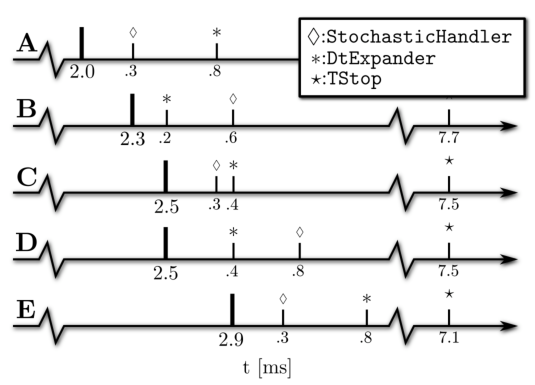
\includegraphics[width=\smallwidth]{chapters/hake/pdf/timeline.pdf}
%  \caption{Diagram for the time stepping algorithm using 3 discrete objects: \texttt{DtExpander}, \texttt{StochasticHandler}, \texttt{TStop}. The values below the small ticks, corresponds to the time to the next event for each of the discrete objects. This time is measured from the last realized event, which is denoted by the thicker tick. In \textbf{A} we have realized a time event at t=2.0 ms. The next event to be realized is a stochastic transition, the one with smallest value below the ticks. In \textbf{B} this event is realized, and the \texttt{StochasticHandler} now show a new next event time. The event is a channel transition forcing the dt, controlled by the \texttt{DtExpander}, to be minimized. \texttt{DtExpander} now has the smallest next event time, and is realized in \textbf{C}. The channel transition that was realised in \textbf{B} raised the \CaC in the cleft which in turn increase the \Ca dependent propensity functions in the included Markov models. The time to next event time of the \texttt{StochasticHandler} has therefore been updated, and moved forward in \textbf{C}. Also note that the \texttt{DtExpander} has expanded its next event time. In \textbf{D} the stochastic transition is realized and updated with a new next event time, but it is ignored as it is not a channel transition. The smallest time step is now the \texttt{DtExpander}, and this is realized in \textbf{E}. In this example we do not realize the \texttt{TStop} event as it is too far away.}
%  \label{fig:time-line}
%\end{figure}
%
%I am combining a solver of the continuous and deterministic advection-diffusion equation, Eq. (\ref{eq:advection-diffusion}), and a solver of the discrete and stochastic systems of Markov chain models from Section \ref{sec:stochastic-models}. These systems are two-way coupled as some of the propensities in the Markov chains are dependent on the local \CaC and boundary fluxes are turned on or off dependent on what state the Markov models are in. I have used a hybrid approach similar to the one presented in \cite{Ruedi_2007_1847} to solve this system. Basically this hybrid method consists of a modified Gillespie method \cite{Gill_1977_2340} to solve the stochastic state transitions, and a finite element method in space together with a backward Euler method in time, to solve the continuous system.\par
%
%\section{\texttt{diffsim} an event driven simulator}
%\label{sec:diffsim}
%In the scripts in Fig.~\ref{fig:assembly-algorithm}-~\ref{fig:solving-algorithm} it is shown how a simple continuous solver can be built with \pydolfin. By pre-assemble the matrices from Eq.~(\ref{eq:matrices}) a flexible system for adding and removing boundary fluxes corresponding to the state of the channels is constructed. The script in Fig.\ref{fig:solving-algorithm} uses fixed time steps for the channel states. These time steps together with an expanding \Dt form a simplistic time stepping scheme that is sufficient to solve the presented example. However it would be difficult to expand it to also incorporate the time stepping involved with the solution of stochastic Markov models, and other discrete variables. For this I have developed an event driven simulator called \texttt{diffsim}. In the last subsections in this chapter I will present the algorithm underlaying the time stepping scheme in \texttt{diffsim} and an example of how one can use \texttt{diffsim} to describe and solve a model of the dyadic cleft. The \texttt{diffsim} software can be freely downloaded from URL:\url{http://www.fenics.org/wiki/FEniCS_Apps}.\par
%
%\subsection{Stochastic system}
%\label{sec:stochastic-system}
%The stochastic evolution of the Markov chain models from Section \ref{sec:stochastic-models} is determined by a modified Gillespie method \cite{Gill_1977_2340}, which resembles the one presented in \cite{Ruedi_2007_1847}. I will not go into detail of the actual method, but rather explain the part of the method that has importance for the overall time stepping algorithm, see below.\par
%
%The solution of the included stochastic Markov chain models is stored in a state vector, \texttt{S}. Each element in \texttt{S} corresponds to one Markov model and the value reflects which state each model is in. The transitions between these states are modelled stochastically and are computed using the modified Gillespie method. This method basically give us which of the states in \texttt{S} changes to what state and when. It is not all such state transitions that are relevant for the continuous system, e.g, a transition between two closed states in the LCC model will not have any impact on the boundary fluxes, and can be ignored. Only transitions that either open or close a channel, which is called channel transitions, will be recognized. The modified Gillespie method assume that any continuous variables a certain propensity function is dependent on are constant during a time step. The error done by assuming this is reduced by taking smaller time steps right after a channel transition, as the continuous field is changing dramatically during this time period. \par
%
%\subsection{Time stepping algorithm}
%\label{sec:event-driven-simulator}
%To simplify the presentation of the time stepping algorithm we only consider one continuous variable, this could for example be the \Ca field. The framework presented here can be expanded to also handle several continuous variables. We define a base class called \texttt{DiscreteObject} which defines the interface for all discrete objects. A key function of a discrete object is to know when its \textit{next event} is due to. The \texttt{DiscreteObject} that has the smallest next event time, gets to define the size of the next \Dt, for which the \Ca field is solved with. In \python this is easily done by making the \texttt{DiscreteObject}s sortable with respect to their next event time. All \texttt{DiscreteObject}s is then collected in a list, \texttt{discrete\_objects} see Fig.~\ref{fig:time-stepping-algorithm}, and the \texttt{DiscreteObject} with the smallest next event time is then just \texttt{min(discrete\_objects)}.\par
%
%An event from a \texttt{DiscreteObject} that does not have an impact on the continuous solution will be ignored, e.g., a Markov chain model transition that is not a channel transition. A transition needs to be realized before we can tell if it is a channel transition or not. This is done by \textit{stepping} the \texttt{DiscreteObject}, calling the objects \texttt{step()} method. If the method returns \texttt{False} it will not affect the \Ca field, and we enter the while loop, and a new \texttt{DiscreteObject} is picked, see Fig.~\ref{fig:time-stepping-algorithm}. However if the object returns \texttt{True} when it is stepped, we will exit the while loop and continue. Next we have to update the other discrete objects with the chosen \Dt, solve the \Ca field, broadcast the solution and last but not least execute the discrete event that is scheduled to happen at \Dt.\par
%
%\editornote{Fix ugly text sticking out in margin.}
%
%In Fig.~\ref{fig:time-line} we show an example of a possible realization of this algorithm. The example starts at t=2ms at the top-most timeline represented by \textbf{A}, and it includes three different types of \texttt{DiscreteObject}s: \texttt{i}) \texttt{DtExpander}, \texttt{ii}) \texttt{StochasticHandler}, and \texttt{iii}) \texttt{TStop}. See the legend of the figure for more details.\par
%\begin{figure}
%  \centering
%  \LVerbatimInput[fontsize=\scriptsize,frame=lines,
%  framerule=0.4mm,
%  xleftmargin=10mm,xrightmargin=15mm,
%  numbers=left,numbersep=5pt]{chapters/hake/code/diffsim_test.py}
%  \vspace{-1.5em}
%  \caption{An example of how \texttt{diffsim} can be used to simulate the time to RyR release latency, from a small dyad whos domain is defined by the mesh in the file \texttt{cleft\_mesh\_with\_RyR.xml.gz}.}
%  \label{fig:diffsim_test}
%\end{figure}
%
%\subsection{\texttt{diffsim} an example}
%\texttt{diffsim} is a versatile event driven simulator that incorporates the time stepping algorithm presented in the previous section together with the infrastructure to solve models with one or more diffusional domains, defined by a computational mesh. Each such domain can have several diffusive ligands. Custom fluxes can easily be included through the framework \texttt{diffsim} give. The submodule dyadiccleft implements some published Markov models that can be used to simulate the stochastic behaviour of a dyad and some convinient boundary fluxes. It also implements the field flux from the lipid bi-layer discussed in Section~\ref{sec:ca-diffusion}. In Fig.~\ref{fig:diffsim_test} runnable script is presented, which simulate the time to release, also called the latency for a dyad. The two Markov models that is presented in section \ref{sec:stochastic-models} is here used to model the stochastic dynamics of the RyR and the LCC. The simulation is driven by an external dynamic voltage clamp. The data that defines this is read in from a file using utilities from the \numpy \python packages.


%In a healthy heart the \Ca release from SR is done in a synchronous way, i.e., it is triggered at the same time and all over the cell. This is important for the effectivness of an heart beat. However during heart failure the TT network is disrupted, causing dyssynchronious release which impairs the quality of the heart beat \cite{Louc_2006_519}. We have modelled the TT disruption by varying the height of the cleft. To measure the effect of the modelled TT disruption on the EC coupling, we made 50 runs for each height and recorded the time it took for a RyR to open. The simulations were done, with and without an electric field, on a cleft with $r = 100$ nm, using the second mesh resolution, see legend in Fig.~\ref{fig:error_plot}. \par

%In Fig.~\ref{fig:boxplot} we present the registered time to release data from our simulations. The left panel shows the time to release results from our simulations without an electric field and the right panel the

%The propensity for a RyR to open is dependent on the local \Ca concentration, see Section \ref{sec:ryr}. This will vary depending on
%\begin{figure}[b]
%    \begin{minipage}[t]{\leftfigsize}
%      \raisebox{-4cm}{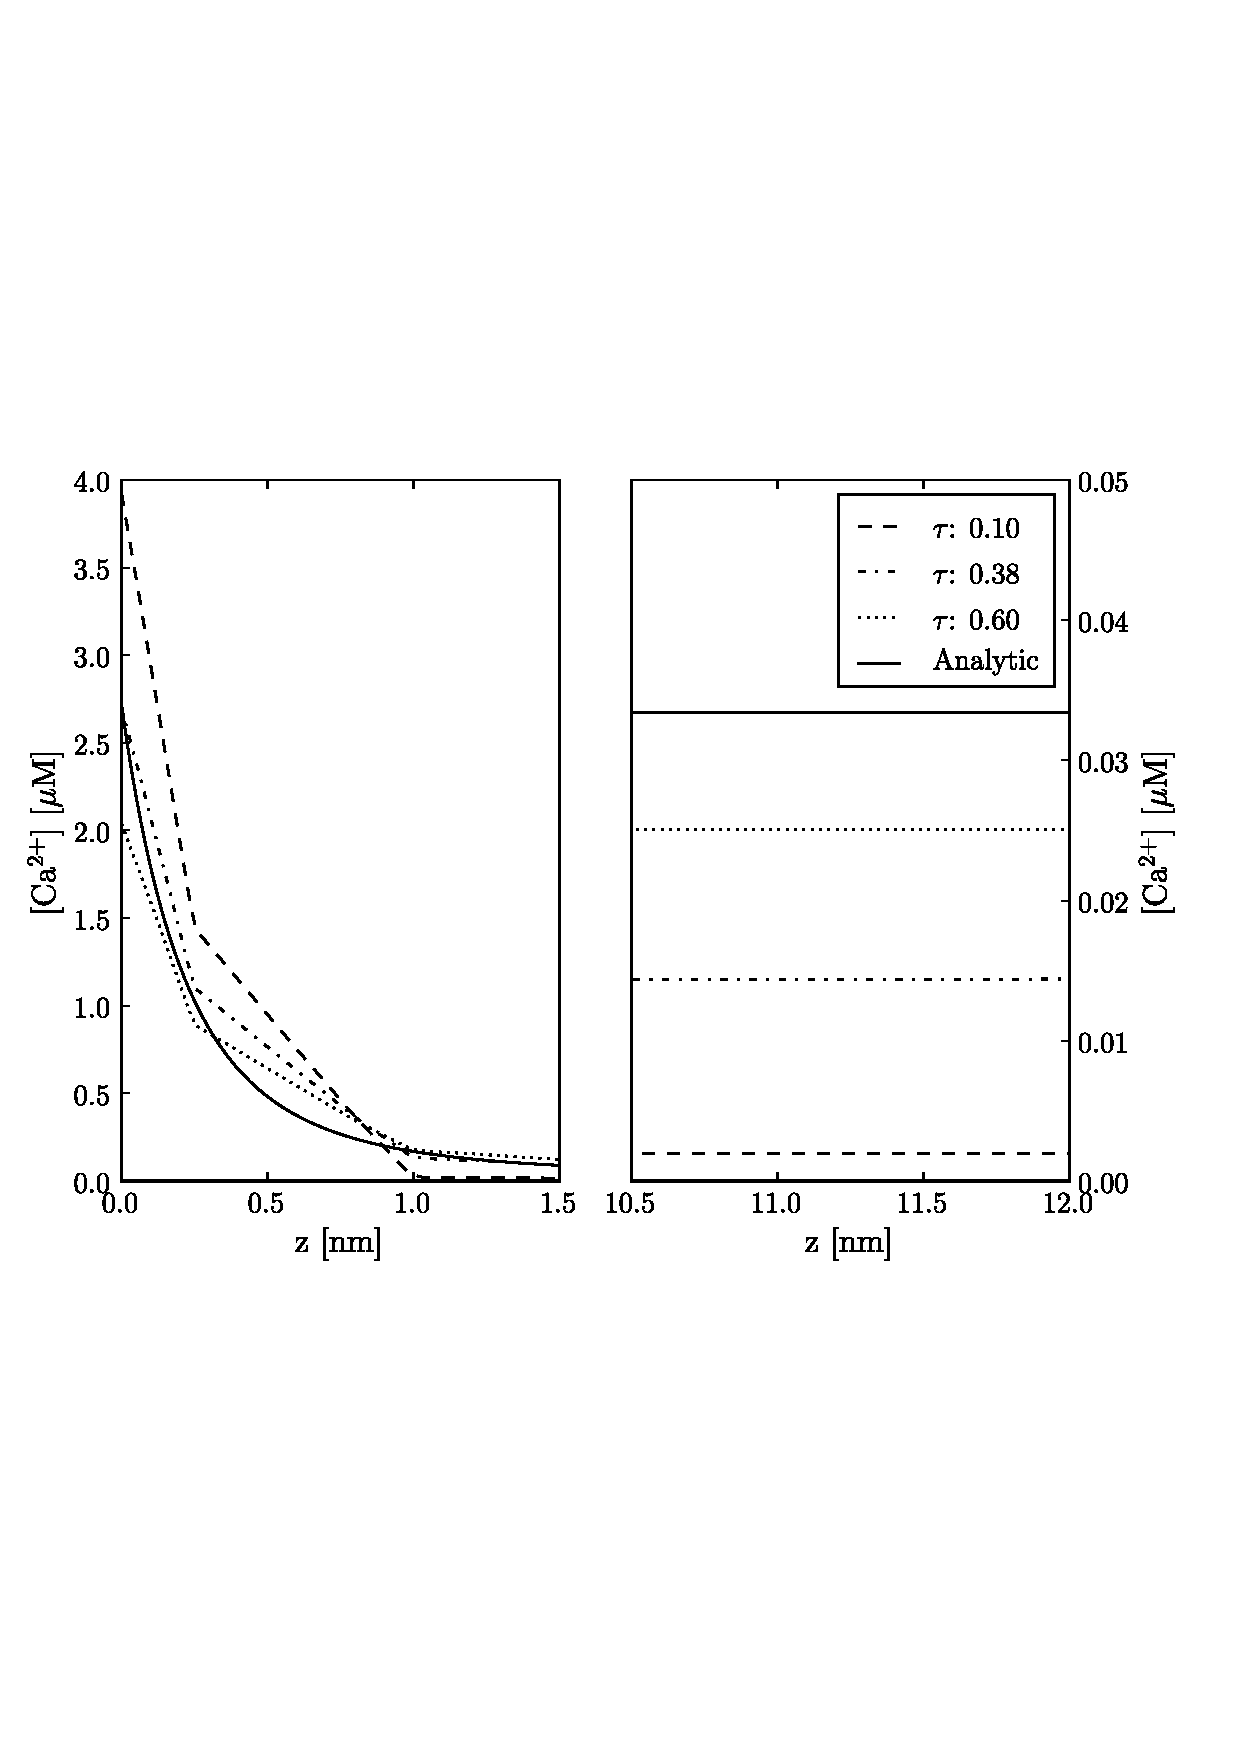
\includegraphics[width=\linewidth]{traces_mesh_3}}
%    \end{minipage}
%    \hfill
%    \begin{minipage}{\rightfigsize}
%      \caption{\captionthree}
%      \label{fig:traces_mesh_3}
%    \end{minipage}
%\end{figure}

%\begin{figure}[t]
%  \centering
%  \includegraphics[width=\linewidth]{tau_results_300}
%  \caption{A figure showing the numerical results for different choice of $\tau$ and mesh resolutions. The 3 mesh resolutions, [0, 1, 2], correspond to mesh with different amount of vertices near the $z=0$. The median of the $z$ distance of all vertices is used to quantitfy the three resolutions: Mesh res 0:0.75nm, Mesh res 1:0.5nm, Mesh res 2:0.25nm. In \textbf{A} we plot the L2 norm of the difference of the analytic and numerical solution, normalized with the size of the domain, against the stabilization parameter $\tau$. We see that the minimal values of the L2 norm, occur at three different $\tau$: 0.22, 0.28, and 0.38. In \textbf{B}-\textbf{D} we have plotted the actual traces of the numerical solution for three different $\tau$ together with the analytic solution. The solutions were picked from a line going betwen (0,0,0) and (0,0,12). In \textbf{B} we plot the whole traces, and in \textbf{C} and \textbf{D} we split each plot into two, sub plots, each showing the traces from the first and last 1.5nm of the plots.}
%  \label{fig:tau_results}
%\end{figure}

%\pagebreak
%\bibliographystyle{biophysic}
%\bibliographystyle{siam}
%\bibliography{heartbib}
%\end{document}

